\chapter{实验设计与结果分析}
本章将详细介绍我们所提出的结合全局路径规划方法和局部路径规划方法的LVL-Nav方法在仿真环境和真实环境下的实验评估结果,包括在仿真环境中不同方法的对比实验来验证本文所提出方法的有效性、针对提出方法的各关键组件进行消融实验分析各个组件的作用和在真实环境中进行目标物体导航的实验。


\section{仿真环境实验设计与评估}
\subsection{数据集}
在仿真实验中,我们使用Gazebo中的离线数据集来进行导航实验以测试我们所提出方法的有效性。Gazebo是一个广泛用于机器人导航控制研究的强大开源仿真环境,它提供了一个高质量的物理引擎来模拟机器人在复杂的环境中的运动、感知、认知和交互,如表\ref{Gazebo与其他仿真环境对比}所示,其中可导航指的是导航代理可以在仿真环境中进行自主移动以探索不同的空间环境;可交互指的是可以手动调整环境中物体的摆放位置或是添加目标物体;物体状态表示环境中的物体会随着时间轴而发生变化,比如钟表会不停地走;动态照明是指随环境中的光源可以动态进行调整,且环境中的物体会随着光源位置的变化而产生不同的阴影;3D资源库指的该仿真环境提供可以添加在环境中不同物体的社区资源;真实对应指的是所使用的仿真世界不是随机生成而是与真实环境一一对应还原的。
相较于其他仿真环境,Gazebo能够提供更全面丰富的可视化系统和导航功能。
\begin{table}
    \caption{\label{Gazebo与其他仿真环境对比}Gazebo与其他仿真环境对比}
    \centering
    \small
    \begin{tabular}{ccccccc}
        \hline
        仿真环境 & 可导航 & 可交互 & 物体状态 & 动态照明 & 3D资源库 & 真实对应 \tabularnewline 
        \hline 
        Gazebo & \checkmark & \checkmark & \checkmark & \checkmark & \checkmark & \checkmark \tabularnewline
        iGibson & \checkmark & \checkmark &  &  &  &  \tabularnewline
        Matterport3D & \checkmark &  &  &  &  &  \tabularnewline
        Minos & \checkmark &  &  &  &  &  \tabularnewline
        Habitat & \checkmark &  &  &  &  &  \tabularnewline
        \hline 
\end{tabular}
\end{table}

在实验的过程中我们使用了类民住房、类酒店、类工厂3种具有不同尺度不同特征的场景,每种类型的场景中都有5个不同样式的环境,环境中共存在有1000多个物体,且每个环境都有120多条自然语言导航指令用于导航测试。自然语言导航指令有单目标、三目标和五目标三种不同的形式,每个环境之下的每种指令都有40多条用于测试导航方法的性能。本文所设计的LVL-Nav方法可以选择32个不同的物体作为导航目标,包括手提电脑、鼠标、花盆、台灯、沙发等室内常见家具。

在全局路径规划过程中,我们通过搭载在移动机器人上的十六线激光雷达在各仿真环境中构建栅格地图,根据所建的栅格地图设置通路中的导航点,并通过ROS导航节点进行导航,记录导航时间构建用邻接矩阵的形式表示的拓扑图。此外,我们获取环境中已经设置的所有导航点的四个方向的位姿信息和对应的视觉观察图像作为全局路径规划导航的依据,用于多模态融合网络模块匹配导航点和目标和执行后续的导航任务。

在局部路径规划过程中,需要获取仿真环境中的特征信息来训练特征提取、特征融合网络模型。具体而言,我们将每个环境都进行网格化,每个网格代表移动机器人能在环境中进行移动的离散动作步,我们将每个到导航点所获得视觉观察送入到预训练的ResNet18网络中提取特征,融合将该导航点的坐标和该点的特征作为键值对进行存储,除此之外,我们还将环境中所存在的所有目标物体的位姿、名称和可以看到该目标物体的导航点作为键值对进行存储。最终获得由导航点、目标物体和最佳动作共同构成的预训练数据集。在训练时,模型首先获得的目标物体名称和当前导航点位姿,然后它会根据导航点所对应的特征输出一个导航动作并和最佳动作计算交叉熵。在不同环境的测试过程中,我们随机给定不同的初始位姿和导航指令。



\subsection{实验参数}%机器人运动参数、多模态融合模块(训练参数) 特征提取、特征融合
在仿真环境中,我们所搭建的移动机器人的运动参数如下表\ref{robotparameter}所示。
\begin{table}
    \caption{\label{robotparameter}机器人运动参数}
    \centering
    \small
    \begin{tabular}{cccccc}
        \hline
        最大线速度 & 最大角速度 & 最大线加速度 & 最大角加速度 & 线速度分辨率 & 角速度分辨率 \tabularnewline 
        \hline 
        0.6${m \mathord{\left/
 {\vphantom {m s}} \right.
 \kern-\nulldelimiterspace} s}$ & 25${^\circ  \mathord{\left/
 {\vphantom {^\circ  s}} \right.
 \kern-\nulldelimiterspace} s}$ &  0.2${{m \mathord{\left/
 {\vphantom {m s}} \right.
 \kern-\nulldelimiterspace} s}^2}$ & 30${{^\circ  \mathord{\left/
 {\vphantom {^\circ  s}} \right.
 \kern-\nulldelimiterspace} s}^2}$  &  0.01${m \mathord{\left/
 {\vphantom {m s}} \right.
 \kern-\nulldelimiterspace} s}$ &  1${^\circ  \mathord{\left/
 {\vphantom {^\circ  s}} \right.
 \kern-\nulldelimiterspace} s}$ \tabularnewline
        \hline 
    \end{tabular}
\end{table}

全局路径规划中的多模态融合网络通过在Interiornet数据集筛选后的20w个数据集进行训练,使用Adam优化器以${10^{ - 4}}$的学习率更新CLIDP网络,我们使用20个异步代理训练5000次episode,每次的batch\_size为128,且每100次保存一次模型数据和精度,然后将得到的模型在划分的验证集里测试精度,最终选取精度最高的模型作为后续导航所使用的模型。
局部路径规划中的特征提取、特征融合模块通过预训练的模型权重进行初始化,使用Adam优化器以${10^{ - 5}}$的学习率更新模型,我们使用20个异步代理训练300万次episode,每10万次保存一次模型数据和精度,然后将得到的30个模型在验证集里测试精度,最终选取精度最高的模型作为后续导航所使用的模型。




\subsection{实验设备}
所有的仿真实验是在笔记本电脑上进行的,模型的训练则是在服务器上进行的,它们的的主要配置参数如表所示\ref{platformconfig}。我们使用双系统的方式在笔记本电脑上安装Ubuntu20.04并搭建ROS所依赖的相关环境,使用VSCode作为代码编辑、环境配置管理和远程连接工具。在服务器上则使用docker容器进行模型训练环境的配置和依赖的安装。
\begin{table}
    \caption{\label{platformconfig}实验平台配置参数}
    \centering
    \small
    \begin{tabular}{ccc}
        \hline
        软硬件 & 服务器配置 & 笔记本电脑配置 \tabularnewline 
        \hline 
        GPU & NVIDIA GeForce RTX 2080Ti × 3 & NVIDIA GeForce RTX 3050Ti \tabularnewline
        CPU & Intel Xeon E5-2620 v4 (32)@3 & AMD Ryzen 9 5900HS \tabularnewline
        内存 & 128GB & 16GB \tabularnewline
        存储 & 4T & 1T \tabularnewline
        操作系统 & Ubuntu18.04 & Ubuntu18.04 \tabularnewline
        开发环境 & Python3.8+Pytorch1.9 & Python3.8+Pytorch1.9 \tabularnewline
        \hline 
    \end{tabular}
\end{table}

仿真差速驱动机器人的建模如图\ref{sim_robot}所示,
\begin{figure}[htbp]
    \centering
    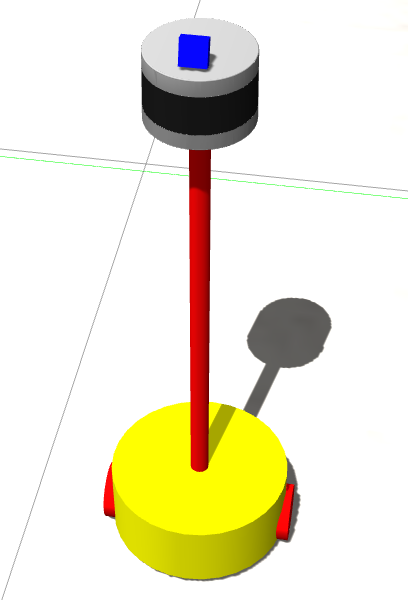
\includegraphics[scale=0.40]{Fig/sim_robot.png}
    \caption{\label{sim_robot}仿真机器人模型}
\end{figure}机器人的底盘由半径为10厘米的圆柱状机身、两个宽度为1.5厘米的驱动论和两个球状万向轮搭建而成,底盘上搭载了一个水平扫描范围为360度、垂直扫描范围30度的十六线激光雷达和单目相机,移动机器人的机身长度为50厘米,宽度为23厘米。
本文在三维动态模拟器Gazebo中进行仿真实验,仿真环境和环境中的点云可视化示例如图\ref{sim_world}所示,为了保证后续不同方法能够进行公平的比较,我们统一使用多线激光SLAM算法扫描各个环境进行全局地图的创建,并且在不同方法的实验过程中均不改变移动机器人上所有设备、ROS导航算法的参数。




\begin{figure}[htbp]
    \centering
    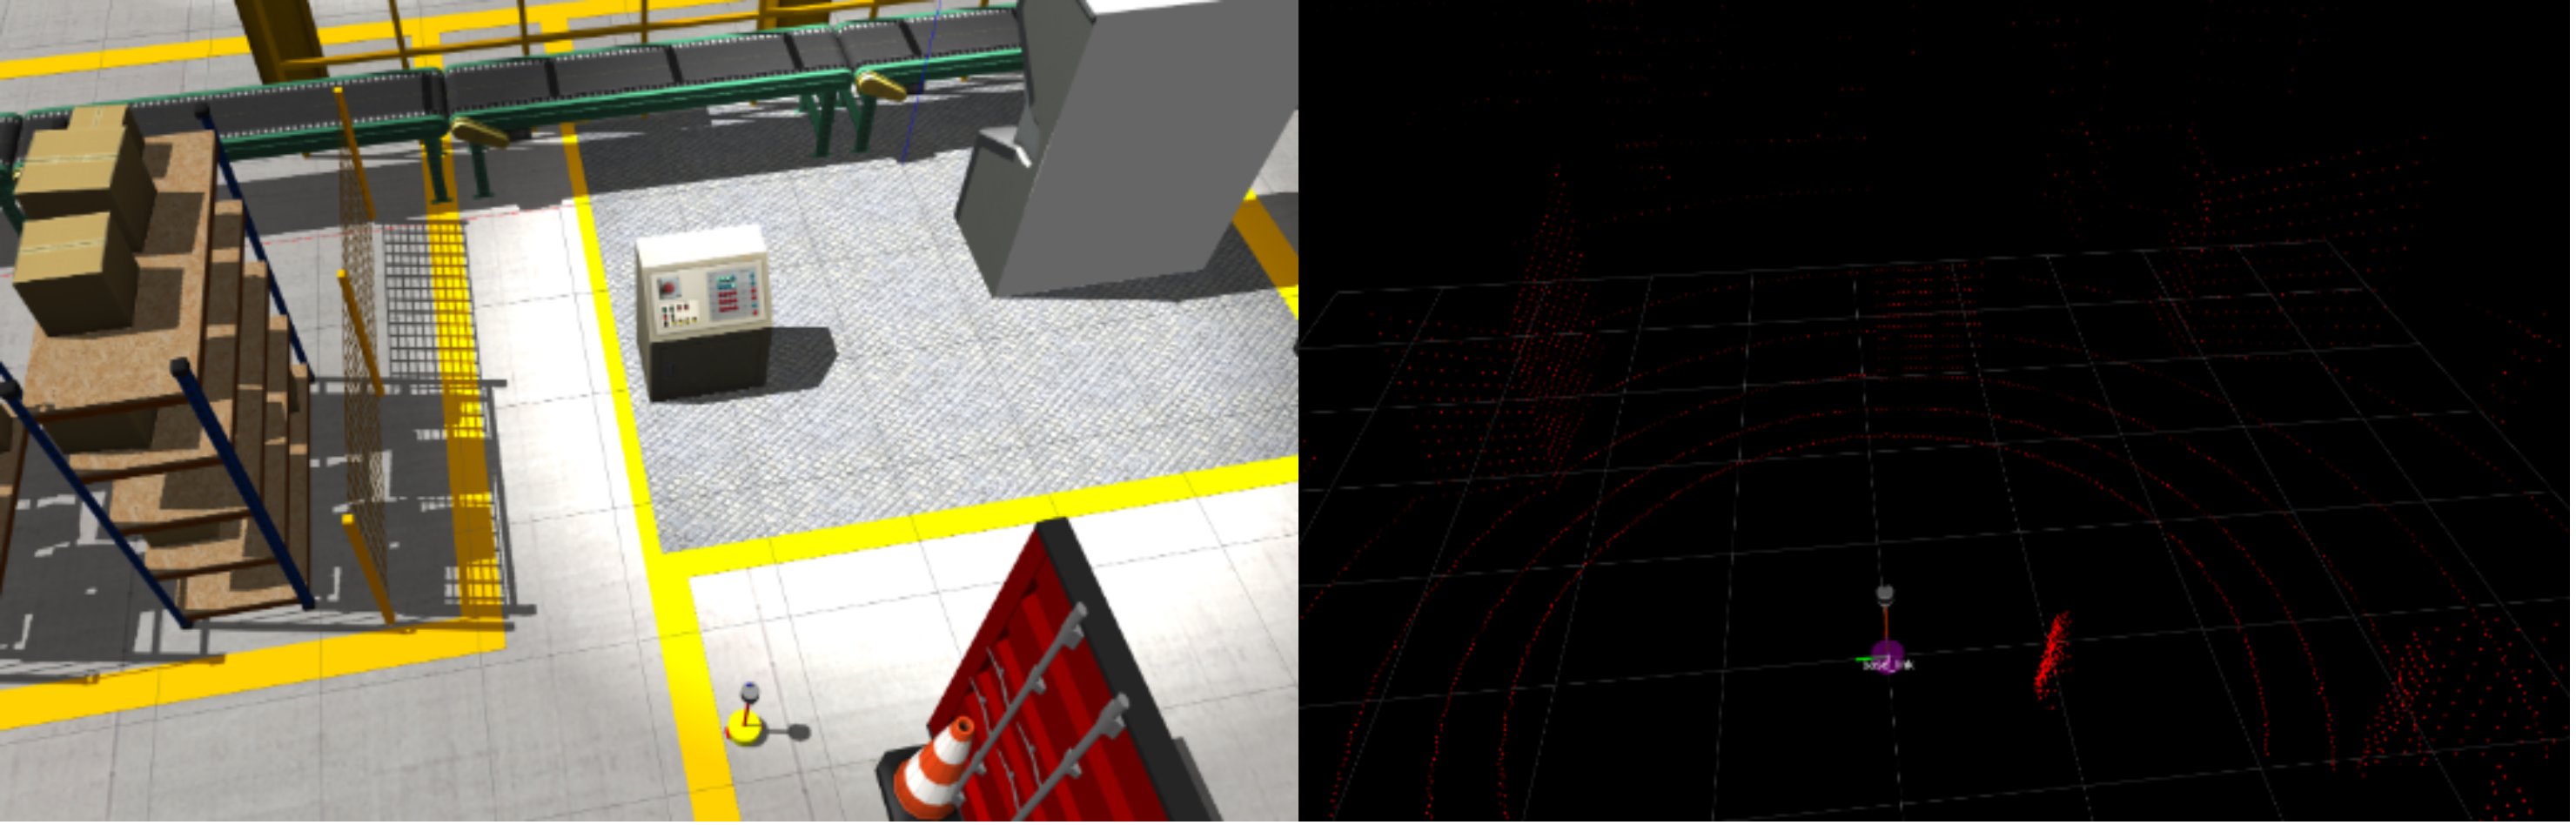
\includegraphics[width=0.95\textwidth]{Fig/sim_world.png}
    \caption{\label{sim_world}仿真环境与可视化点云}
\end{figure}


\subsection{评价指标}
本文通过导航成功率(SR)、导航路径匹配度(PMD)和导航效率(SPL)三个方面来评估导航方法的综合性能,SR衡量导航的有效性,MD衡量导航符合指令要求的程度,SPL衡量导航效率,其具体表达公式如下。
\begin{enumerate}[topsep = 0 pt, itemsep= 0 pt, parsep=0pt, partopsep=0pt, leftmargin=44pt, itemindent=0pt, labelsep=6pt, label=(\arabic*)]
    \item 	\textbf{成功率(Success Rate, SR)}。成功率指移动机器人根据自然语言指令进行导航的过程中,成功完成导航所占的比例,取值范围从0到1。
    \begin{equation}
        SR = \frac{1}{N}\sum\limits_{n = 1}^N {{S_n}} 
        \label{myeq51}
    \end{equation}
    其中$N$表示导航总次数,${S_n}$表示执行第n次导航的指标,导航成功时值为1,导航失败时值为0。
    \item	\textbf{路径匹配度(Path Matching Degree, PMD)}路径匹配度指移动机器人根据自然语言指令进行导航的过程中,依次经过的目标与指令要求的目标相匹配所占的比例,取值范围从0到1。
    \begin{equation}
        PMD = \frac{1}{{N \cdot M}}\sum\limits_{n = 1}^N {\left( {\sum\limits_{m = 1}^M {{a_{nm}}} } \right)} 
        \label{myeq53}
    \end{equation}
    其中$M$表示导航指令中存在的目标个数,$a_{nm}$表示导航子目表匹配指标,导航点匹配时值为1,导航点不匹配时值为0。
    \item	\textbf{成功路径长度加权比率(Success weighted by Path Length, SPL)}。成功路径长度加权比率指移动机器人根据自然语言指令进行导航的过程中,根据实际执行路径和最优路径的关系从0到1取值,当实际执行路径与导航最优路径越接近则取值越高,代表导航的效率越高。
    \begin{equation}
SPL = \frac{1}{N}\sum\limits_{n = 1}^N {\left( {{S_n} \cdot \left( {\frac{{{T_n}}}{{{t_n}}}} \right)} \right)} 
        \label{myeq53}
    \end{equation}
    其中$T_{n}$表示完成第n次导航时所需的最短时间,$t_{n}$表示完成第n次导航时的实际耗时。
\end{enumerate}






\subsection{对比实验}

\subsubsection{对比方法}
\begin{enumerate}[topsep = 0 pt, itemsep= 0 pt, parsep=0pt, partopsep=0pt, leftmargin=44pt, itemindent=0pt, labelsep=6pt, label=(\arabic*)]
    \item 	Random Policy:随机策略模型的代理在随机的时间步中,根据平均的概率分布去选择动作空间中的动作进行执行,或是直接在环境中停止以结束导航任务。
    \item	Baseline:基准导航策略直接将局部路径规划中的特征提取得到的局部、全局和目标特征直接送入LSTM网络进行离散动作推理。用于对比验证本文所提出方法中特征融合模块的作用。
    \item   CLIP\cite{radford2021learning}:CLIP基于对比学习的方法提出了一种多模态融合的网络结构,通过有效地将图像和文本信息结合在一起来提供更强的跨模态理解能力,克服了传统模型依赖单一数据源的缺陷,使移动机器人能够理解环境中的目标物体和语义信息以指导导航任务的执行。
    \item   EONS\cite{electronics11071136}:EONS借助ROS框架提出了一种有效的目标导航策略。首先对常见的室内物体进行语义关联分析,利用Mask R-CNN和残差连接网络建立物体语义关联模型,通过ROB-SLAM系统方法构建了一个高可用性的环境图,在移动机器人导航的过程中寻找可达的最优路径以完成导航。
    \item	ViNG\cite{shah2021ving}:与传统的基于地图或几何推理的导航方法不同,ViNG提出了一种创新的视觉语言导航方法,通过学习如何从视觉目标图像中推断导航策略和先前观察到的数据构建环境的拓扑图,通过导航点建议(Waypoint Proposal)、拓扑图剪枝(Graph Pruning)和负挖掘(Negative Mining)多种核心策略,使机器人能够根据目标图像和环境拓扑图在现实世界环境中实现高效率的自主导航。
    \item	LM-Nav\cite{shah2023lm}:LM-Nav通过三个大型预训练模型协同合作,完成了移动机器人根据自然语言指令进行导航的全部流程,包括负责将用户输入的自然语言指令转化为具有顺序的目标序列大语言模型GPT3、负责将目标序列与环境地图中的节点进行特征关联以建立具有先后导航顺序的导航点视觉语言模型(VLM)和负责构建环境拓扑图并利用凸优化技术规划从起点到终点最优路径的视觉导航模型(VNM)。
    \item	LVL-Nav(Ours):提出了一种多模态融合的导航方法,将导航过程拆分成全局和局部路径规划两个部分。通过引入深度信息优化传统的视觉语言模型,提出一种方位优化算法筛选不符合方位条件的冗余导航点,结合导航点规划算法进一步提高全局路径规划中导航点的正确率,再通过特征提取、融合网络在局部未知环境中进行探索,最后由图像点云融合模块完成目标物体导航任务。
	
\end{enumerate}

\subsubsection{对比结果}
在和近三年流行方法的对比试验如表\ref{cmpresult}所示。本文所提出的方法的导航指标在五目标的导航测试指令中的成功率SR(77.4\%)、路径匹配度PDM(77.4\%)和成功路径长度加权比率(62.1\%)三个指标中的性能表现都是最好的。在与五目标指令的基准模型的对比中,本文所提出方法的成功率SR(+22.9\%)、路径匹配度PDM(+23.5\%)和成功路径长度加权比率(+22.6\%)三个指标都大大超过了基准模型。在五目标指令实验中与当前表现最好的LM-Nav模型相比,本文的方法在成功率SR(+1.9\%)、路径匹配度PDM(+3.5\%)和成功路径长度加权比率(+8.7\%)三个指标上也都有所提升,这是因为我们在全局路径规划中通过引入深度信息优化多模态融合网络,提高模型在光线条件变化大的室内的鲁棒性,提出了一种方位优化法,结合指令中提供的方位信息与移动机器人的实时位姿,筛选不符合方位条件的冗余导航点,再通过导航点规划算法进一步提高全局路径规划所生成导航点的正确率,然后在局部路径规划中我们设计了一种特征提取、融合网络能够有效地在局部未知环境中进行探索,设计并实现了一种单目相机和多线激光传感器融合的局部导航方法,以完成导航至目标半米内的闭环任务,这表明了我们所提出方法的有效性。
\begin{table}[]
\caption{\label{cmpresult}实验定量结果对比}
\centering
    \begin{tabular}{c|ccc|ccc|ccc}
    \hline
    \multirow{2}{*}{Methhod} & \multicolumn{3}{c|}{I=1} & \multicolumn{3}{c|}{I=3} & \multicolumn{3}{c}{I=5}                 \\ \cline{2-10} 
                             & SR     & PMD    & SPL    & SR     & PMD    & SPL    & SR   & PMD  & SPL                       \\ \hline
    Ramdom                   & 6      & 6      & 3.9    & 0      & 0      & 0      & 0    & 0    & 0                         \\
    CLIP                     & 66.2   & 66.2   & 65.3   & 42.2   & 43.7   & 64.9   & 32.7 & 36.5 & 60.6                      \\
    Baseline                 & 73.1   & 73.1   & 48.3   & 67.4   & 69.5   & 45.8   & 51.8 & 53.9 & 39.5                      \\
    EONS                     & 78.5   & 78.5   & 31.7   & 75.0   & 76.8   & 29.4   & 64.1 & 65.5 & 26.2                      \\
    ViNG                     & 82.6   & 82.6   & 63.3   & 79.3   & 78.9   & 62.2   & 70.7 & 71.1 & 59.0                      \\
    LM-Nav                   & 85.3   & 85.3   & 57.6   & 79.4   & 77.1   & 54.9   & 72.8 & 73.9 & 53.4                      \\ \hline
    \textbf{Ours}            & \textbf{88.4}   & \textbf{88.4}   & \textbf{66.7}   & \textbf{82.3}   & \textbf{82.9}   & \textbf{65.2}   & \textbf{74.7} & \textbf{77.4} & \textbf{62.1} \\ \hline
    \end{tabular}
    \label{cmpresult}
    \end{table}


相比于我们所提出的方法,CLIP将图像和文本嵌入同一空间中来判断导航目标,但在动态变化的室内环境中容易发生物体移动、光线变化等情况,或是环境中的多个位置都存在相同的目标物体时,该模型缺乏足够的动态适应和区分不同方向正确目标的能力,无法有效地将导航点与目标做出正确的匹配从而导致导航失败,这导致该方法在导航成功率方面的指标表现不佳。

EONS借助构建的语义关联模型在环境中通过直接寻找目标物体或是与目标最相关联的物体从而引导代理执行导航任务。但这种方法依赖于训练过程中环境物体之间的固定关联信息,在静态的环境中表现较为出色,但对于存在多种移动物体的动态环境中,这种目标导航策略无法及时更新目标位置和状态,从而引发导航的错误。除此之外,当EONS在导航过程中未能第一时间观察到目标时,会根据关联模型寻找关联性最强的物体进行探索,这种探索策略占用了大部分的导航时间,导致该方法在导航效率方面的指标表现不佳。

ViNG通过结合视觉目标学习和构建环境拓扑图实现了基于视觉的目标导航,因此在导航效率指标上取得了不错的结果,但是它过度依赖于视觉目标的识别的定位,在很有可能出现遮挡或曝光、欠曝的复杂的室内环境中容易导致目标识别失败,模型无法正确的指导代理进行有效的探索从而导致导航任务的失败。这导致该方法在导航成功率方面的指标表现不佳。

LM-Nav通过大语言模型有效的解析导航任务,利用大量导航数据训练视觉语言模型和视觉导航模型,在多种复杂环境中指导代理生成正确的导航动作,这种联合多种大模型在环境中执行导航任务的方式具有一定的有效性,但这种导航方法在执行任务的过程中依赖于模型的推理速度,等待各种大模型响应的时间占据了部分的导航时间,因此它的导航效率并不高。

LM-Nav在实验中取得了次优的结果,该方法与我们所提出的LVL-Nav导航方法在根据不同指令执行导航任务时的轨迹结果如图\ref{LM-NavcmpLVL-Nav}所示,
\begin{figure}[htbp]
    \centering
    %\includegraphics[width=3in]{fig5}
    \subfloat[类家庭仿真环境下的导航]{
            \includegraphics[width=0.9\textwidth]{Fig/cmp-small-house.drawio.png}
            \label{LM-NavcmpLVL-Nava}}\\
    \subfloat[类工厂仿真环境下的导航]{
            \includegraphics[width=0.9\textwidth]{Fig/cmp-factory.png}
            \label{LM-NavcmpLVL-Navb}}\\
    \subfloat[类医院仿真环境下的导航]{
            \includegraphics[width=0.9\textwidth]{Fig/cmp-hospital.png}
            \label{LM-NavcmpLVL-Navc}}
    \caption{LM-Nav和LVL-Nav路径对比图}
    \label{LM-NavcmpLVL-Nav}
\end{figure}
其中$S$表示随机初始化的移动机器人起点,标号$1,2,...,5$分别表示算法根据指令所执行经过的子目表导航点,$D$表示本文提出方法中局部路径规划获得的导航终点。具体来说,在类家庭仿真环境\ref{LM-NavcmpLVL-Nava}中LM-Nav方法无法正确匹配到曝光状态下的沙发,引导移动机器人移动至错误的导航点,而本文提出的LVL-Nav则通过引入深度信息提高模型在曝光或欠曝的室内环境中的鲁棒性,在全局路径规划中正确地匹配到了曝光状态下的沙发;在\ref{LM-NavcmpLVL-Navb}、\ref{LM-NavcmpLVL-Navc}中LM-Nav方法无法正确避免环境中所存在的其他相似物体影响导航的规划,当指令要求移动到路障或椅子旁时,将移动机器人引导至错误的导航点,而本文所提出的方位优化法能够结合指令中提供的方位信息与移动机器人的实时位姿,筛选不符合方位条件的冗余导航点,在全局路径规划中正确地匹配指令所指方向的目标。图\ref{LM-NavcmpLVL-Nav}和表\ref{cmpresult}统计的结果表明,本文所提出的方法不依赖于导航点的初始化,能够在动态变化复杂环境中指导代理正确地匹配导航点,在局部路径规划部分高效执行探索动作并可靠地完成导航至目标半米内的闭环任务。







在对比实验的过程中,我们把本文全局路径规划中的多模态融合方法和LM-Nav方法在训练过程中每200个epoch保存一次的模型在验证集上测试精度,如图\ref{curvecmp}所示。
\begin{figure}[htbp]
    \centering
    \subfloat[成功率]{
            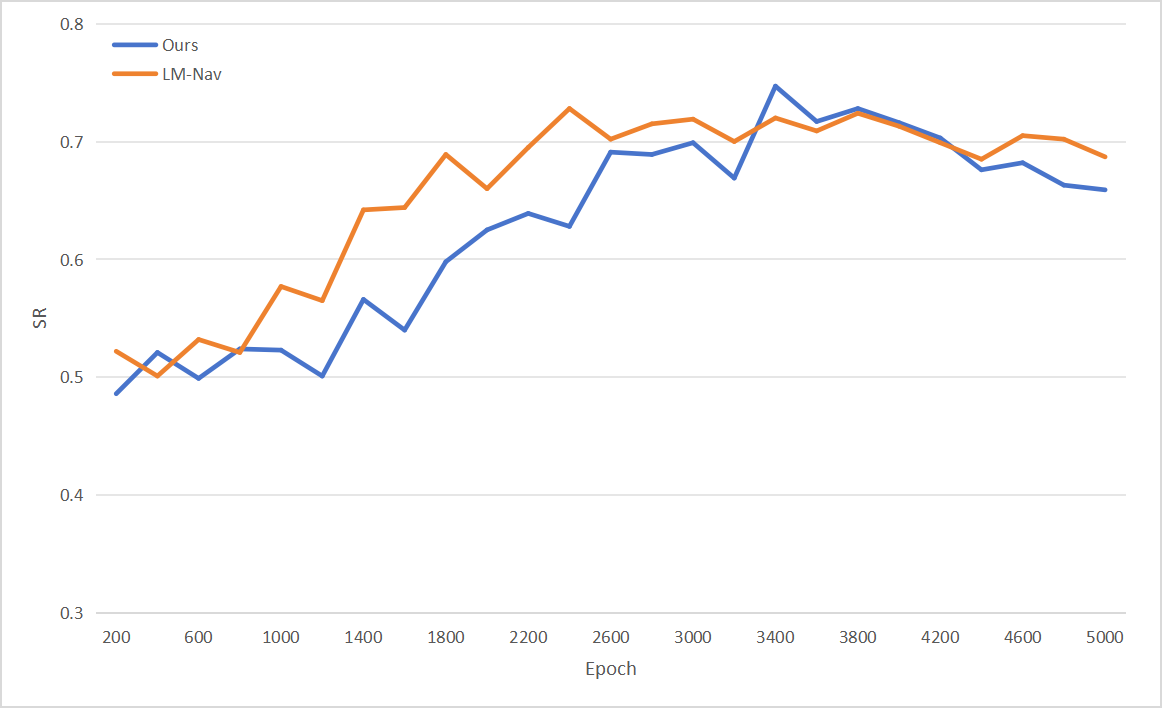
\includegraphics[width=0.9\textwidth]{Fig/curvecmp.png}}\\
    \subfloat[路径匹配度]{
            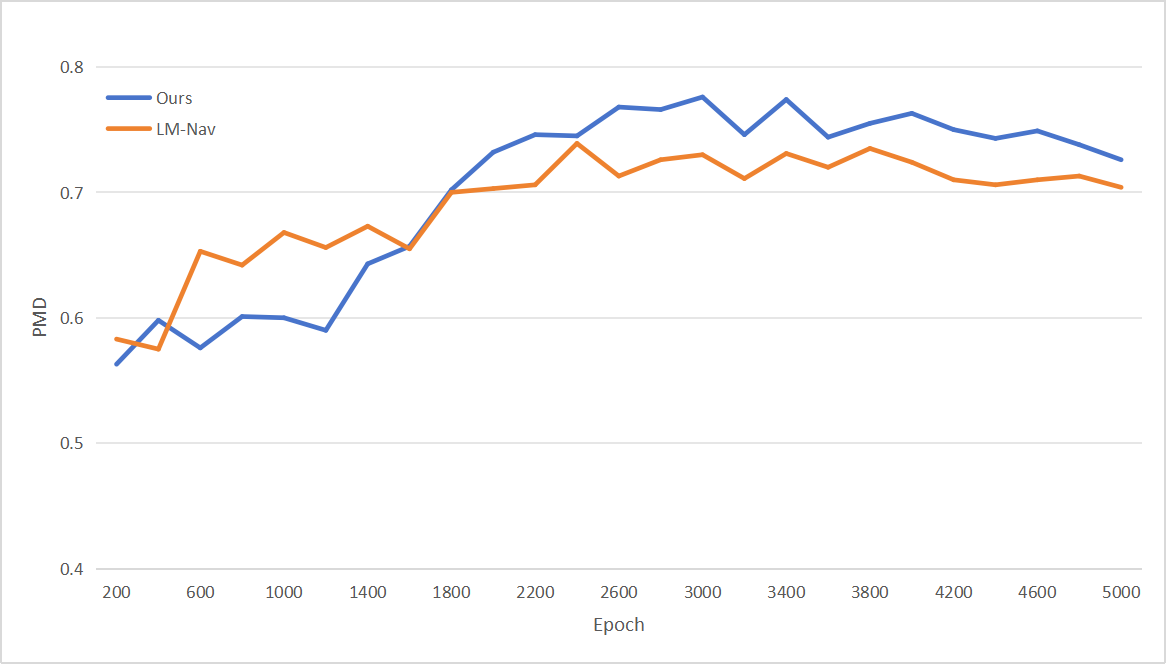
\includegraphics[width=0.9\textwidth]{Fig/curvecmp2.png}}
    \caption{导航指标变化图}
    \label{curvecmp}
\end{figure}
将两种方法在测试集上的成功率SR和路径匹配度PMD进行对比,可以发现本文提出的方法在经过足够的训练后的表现优于LM-Nav。本方法的模型中添加了深度图特征提取架构,学习的速度会更慢,我们的方法在第1800个epoch时的SR只有59.8\%,而LM-Nav方法则达到了68.9\%(+9.1\%)。此外,我们的方法在训练的过程中收敛更慢,在第2400个epoch时LM-Nav方法基本收敛到精度最高值,而我们的方法则在3400个epoch时候才基本收敛到精度最高值。另一方面,我们的方法在3400次epoch后得到的成功率最高值74.7\%(+1.9\%)比LM-Nav方法的成功率最高值72.8\%在测试集上的表现会更好;我们的方法在1800次epoch后得到的路径匹配度比LM-Nav方法的路径匹配度在测试集上表现得更好,并在第3400次epoch后得到路径匹配度最高值77.4\%(+3.5\%)比LM-Nav方法得路径匹配度最高值73.9\%匹配度更高,这得益于我们提出的多模态融合网络框架能够结合深度特征信息归纳表征视觉观察和目标物体文本特征,能够在复杂光照条件下正确通过利用深度信息进行图像-文本匹配,从而提升导航的成功率。




\subsection{消融实验}

为了逐步验证本文所提出的多模态融合网络、导航点规划、方位优化和局部路径规划算法的有效性,我们对上述各关键模块进行仿真消融实验。我们在仿真环境下进行的消融实验中依次添加多模态融合模块、导航点规划算法、方位优化算法、局部路径规划算法来测试各个模块对于指导代理进行高效且正确地导航的有效性,根据他们分别执行基于自然语言指令后记录的评价指标结果如表\ref{Ablationtable}所示,我们分析了各模块的作用。

\begin{table}[]
    \caption{\label{Ablationtable}消融实验结果}
    \centering
        \begin{tabular}{cc|c|c|c|c}
        \hline
        \multicolumn{2}{c|}{Method}                     & +多模态融合 & +导航点规划 & +方位优化 & +局部路径规划 \\ \hline
        \multicolumn{1}{c|}{\multirow{2}{*}{I=1}} & SR  & 66.2   & 78.3   & 83.4  & \textbf{88.4}    \\
        \multicolumn{1}{c|}{}                     & SPL & 65.3   & 54.0   & 62.7  & \textbf{66.7}    \\ \hline
        \multicolumn{1}{c|}{\multirow{3}{*}{I=5}} & SR  & 49.6   & 60.9   & 68.1  & \textbf{74.7}    \\
        \multicolumn{1}{c|}{}                     & PMD & 51.9   & 61.7   & 69.4  & \textbf{77.4}    \\
        \multicolumn{1}{c|}{}                     & SPL & 59.3   & 46.6   & 57.2  & \textbf{62.1}    \\ \hline
        \end{tabular}
    \end{table}

\begin{enumerate}[topsep = 0 pt, itemsep= 0 pt, parsep=0pt, partopsep=0pt, leftmargin=44pt, itemindent=0pt, labelsep=6pt, label=(\arabic*)]
    \item 	多模态融合模块:我们直接使用多模态融合网络进行指令目标与导航点之间的匹配,并将匹配的结果直接发布至/move\_base\_simple话题之中交由ROS导航节点执行导航。实验结果表明在单目标指令中成功率SR(-22.2\%)成功路径长度加权比率(-1.4\%),在五目标指令中成功率SR(-25.1\%)、路径匹配度PDM(-25.5\%)和成功路径长度加权比率(-2.8\%),由于缺失了导航点规划算法所引入的加权最短距离算法,忽略了自然语言指令导航所具有循序渐进的特性,使该导航方法只能锁定环境中与指令目标最相像目标从而导致导航的失败。
    \item	导航点规划算法:我们在全局路径规划中的多模态融合模块基础之上引入了导航点规划算法,将算法匹配的导航点序列交由ROS节点执行导航。实验结果表明单目标指令中成功率SR(-10.1\%)成功路径长度加权比率(-12.7\%),在五目标指令中成功率SR(-13.8\%)、路径匹配度PDM(-15.7\%)和成功路径长度加权比率(-15.5\%),导航点规划算法能依赖于指令目标与环境匹配的相似度和拓扑图中的距离进行规划,相比单纯的多模态融合算法在导航成功率上提升了很多,但当环境中的不同位置存在多个相同目标的环境时,该导航方法无法根据指令信息筛选掉错误的导航点从而导致导航的失败,且该规划算法计算开销大,导航效率很低。
    \item   方位优化算法:我们将完整的全局路径规划算法直接进行实验,将算法匹配的导航点序列交由ROS节点执行导航。实验结果表明单目标指令中成功率SR(-5.0\%)成功路径长度加权比率(-4.0\%),在五目标指令中成功率SR(-6.6\%)、路径匹配度PDM(-8.0\%)和成功路径长度加权比率(-4.9\%),首先方位优化算法能够有效的剔除不再指令要求方位上的相似目标,该方法在具有多个相同目标的环境中进行导航尤为出色,并且方位优化算法能提前筛洗大部分的待规划导航点以减少导航点规划算法的计算开销,大幅地提高了导航效率。但这种方法受限于环境中导航点的初始化设置,当导航点中未能出现目标或是导航点未能设置在目标半米之内的时候会导致导航的失败。
    \item   局部路径规划:添加了由特征提取、融合和图像点云融合模块的局部路径规划方法让代理能够在导航点中未能出现目标的情况下进行局部范围内的自主探索,并在探索的过程中锁定目标,然后通过图像点云融合模块将激光雷达感知和视觉观察认知信息相结合,以获得目标的最终位姿,在进行坐标变换之后发布导航即可完成完整的目标物体导航任务。
\end{enumerate}

消融实验的结果表明多模态融合模块、导航点规划算法、方位优化算法、局部路径规划算法均能有效地提高移动机器人的导航成功率、导航匹配度和导航效率,且随着指令中目标数量的增多,本文提出的LVL-Nav方法具有更高的导航匹配度和导航成功率。


在消融实验过程中取出一组五目标指令下进行导航的结果如图\ref{Ablationfig}所示。
\begin{figure}[htbp]
    \centering
    \subfloat[多模态融合导航路径]{
            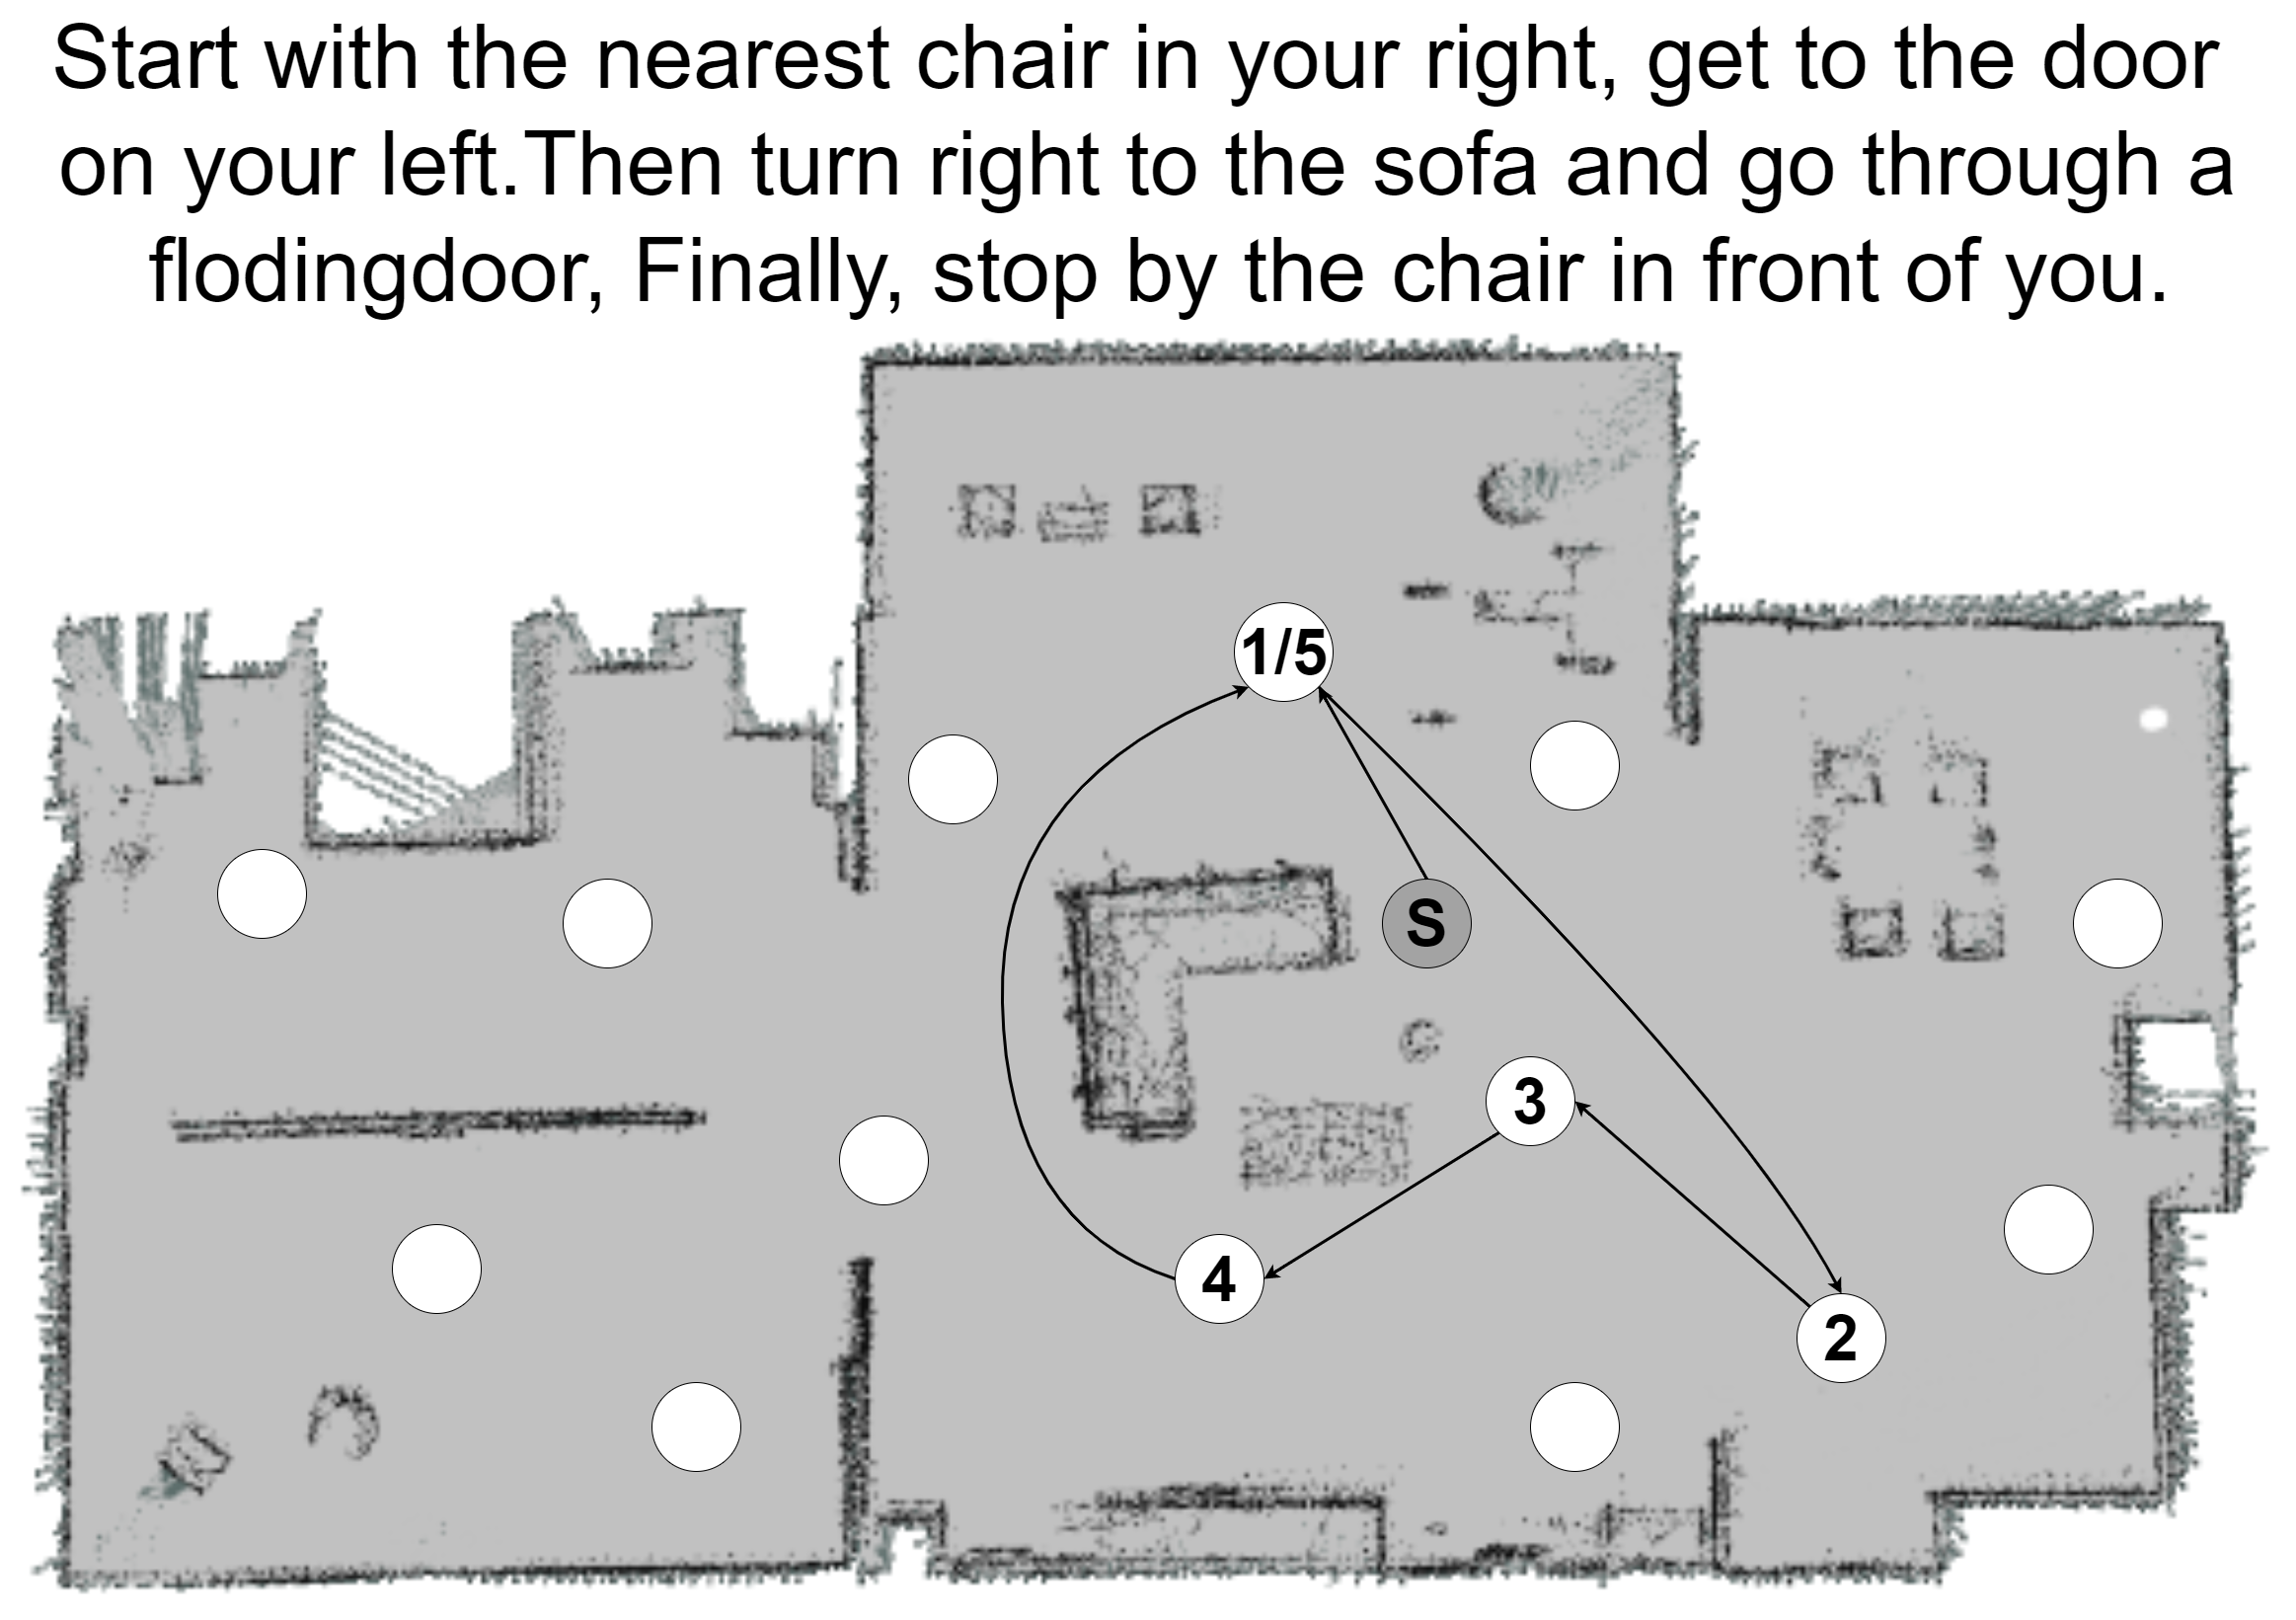
\includegraphics[width=0.5\textwidth]{Fig/消融a.png}
            \label{Ablationfiga}}\\
    \subfloat[多模态融合+导航点规划导航路径]{
            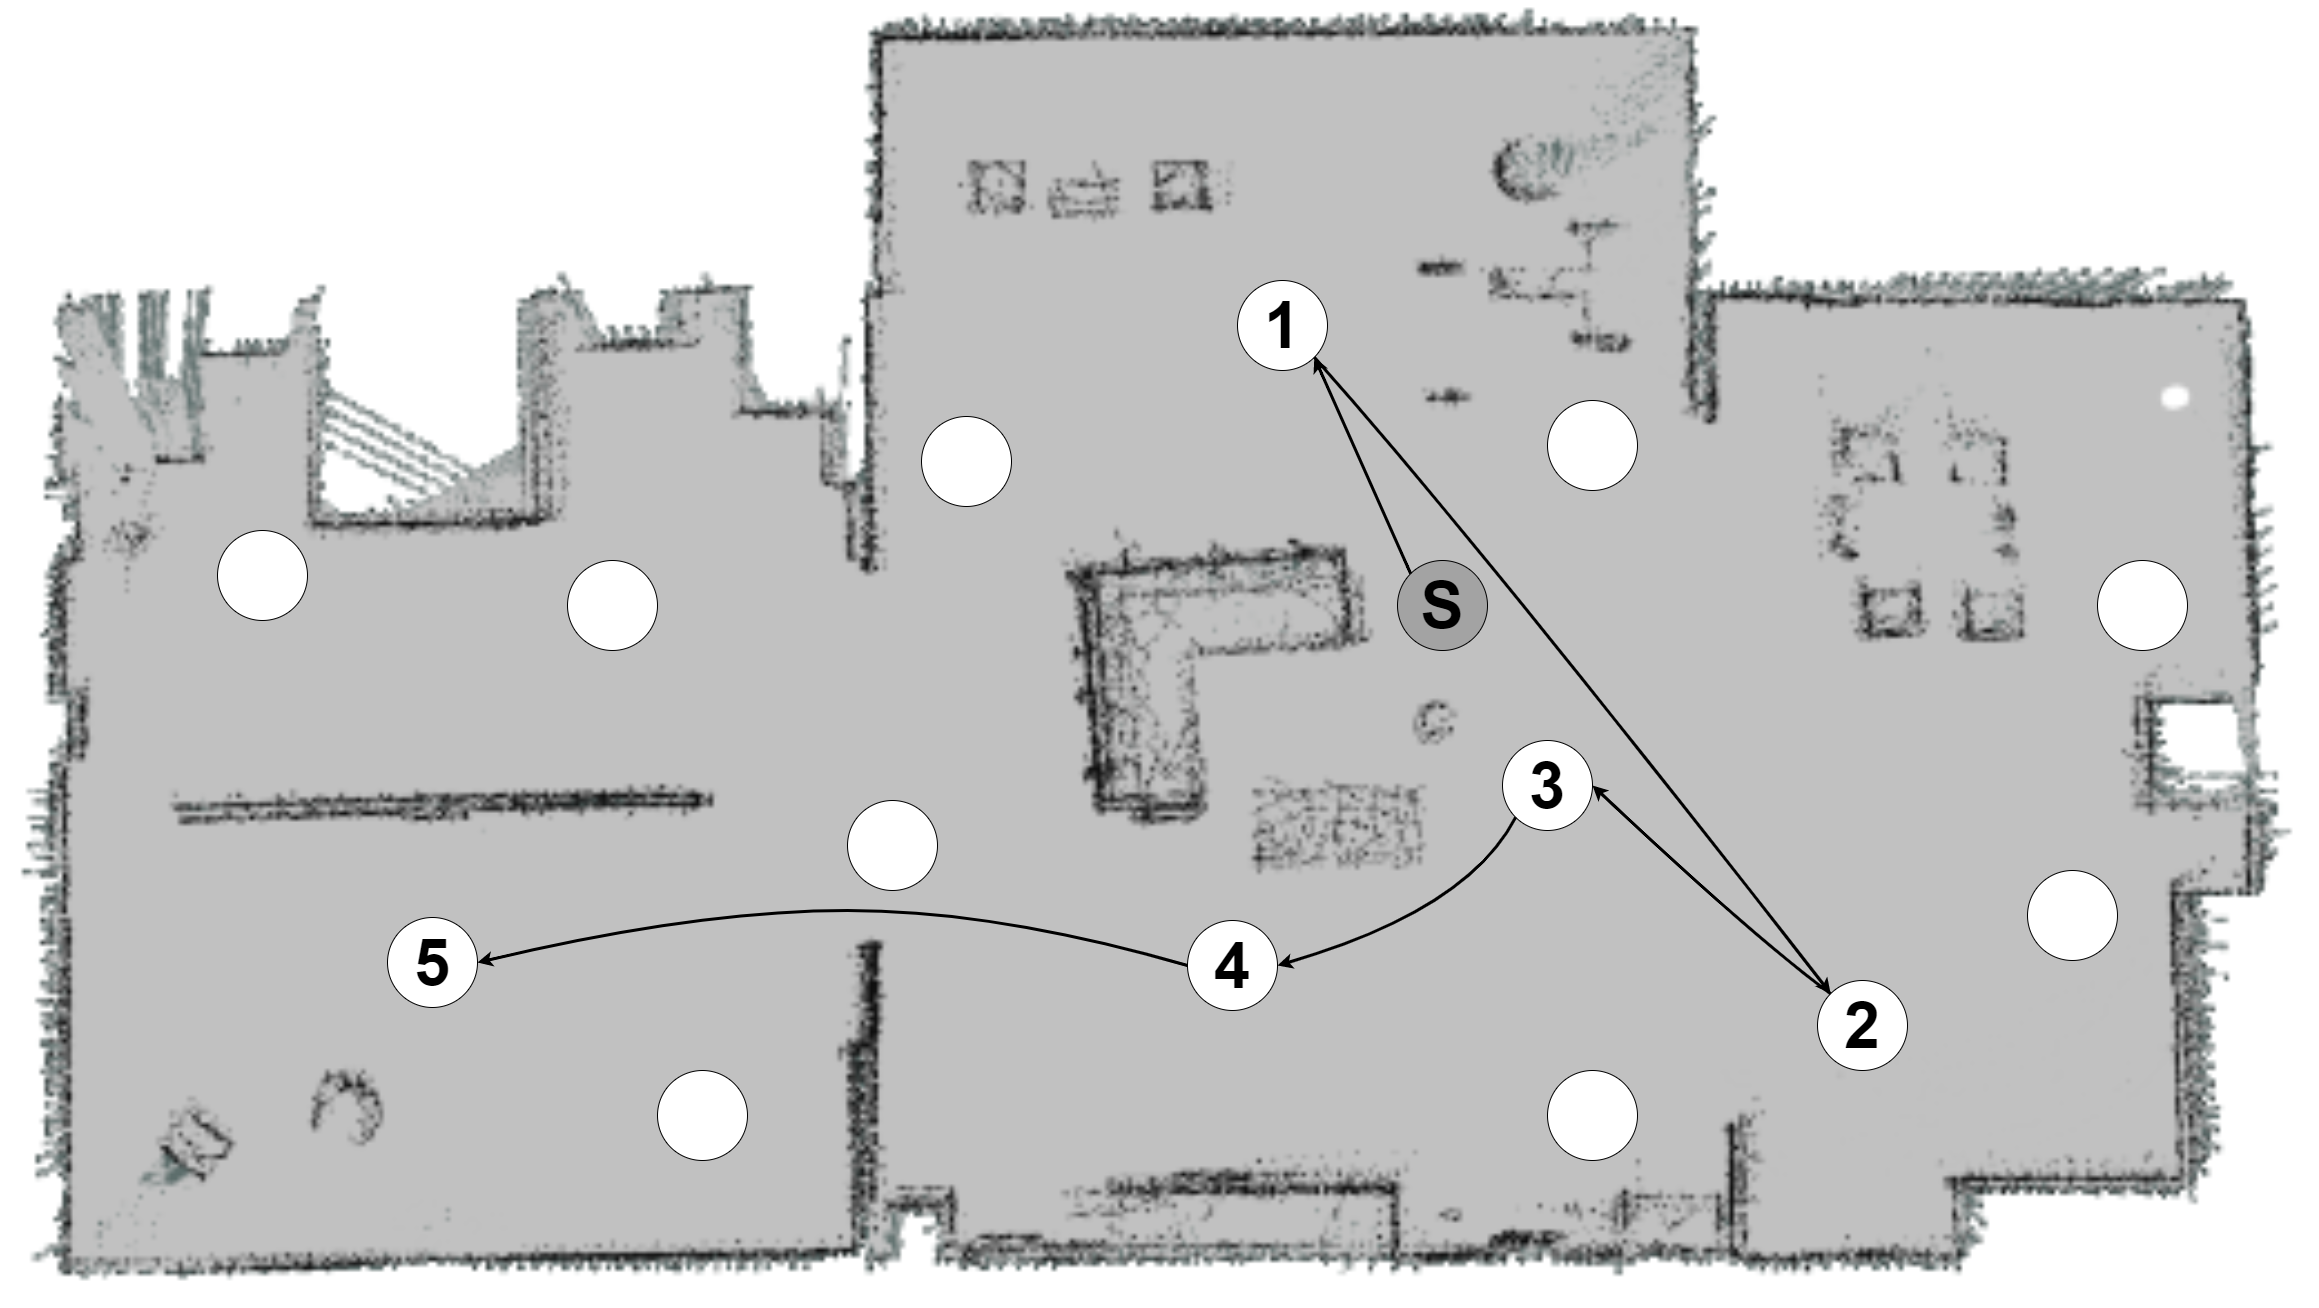
\includegraphics[width=0.5\textwidth]{Fig/消融b.png}
            \label{Ablationfigb}}\\
    \subfloat[多模态融合+导航点规划+方位优化导航路径]{
            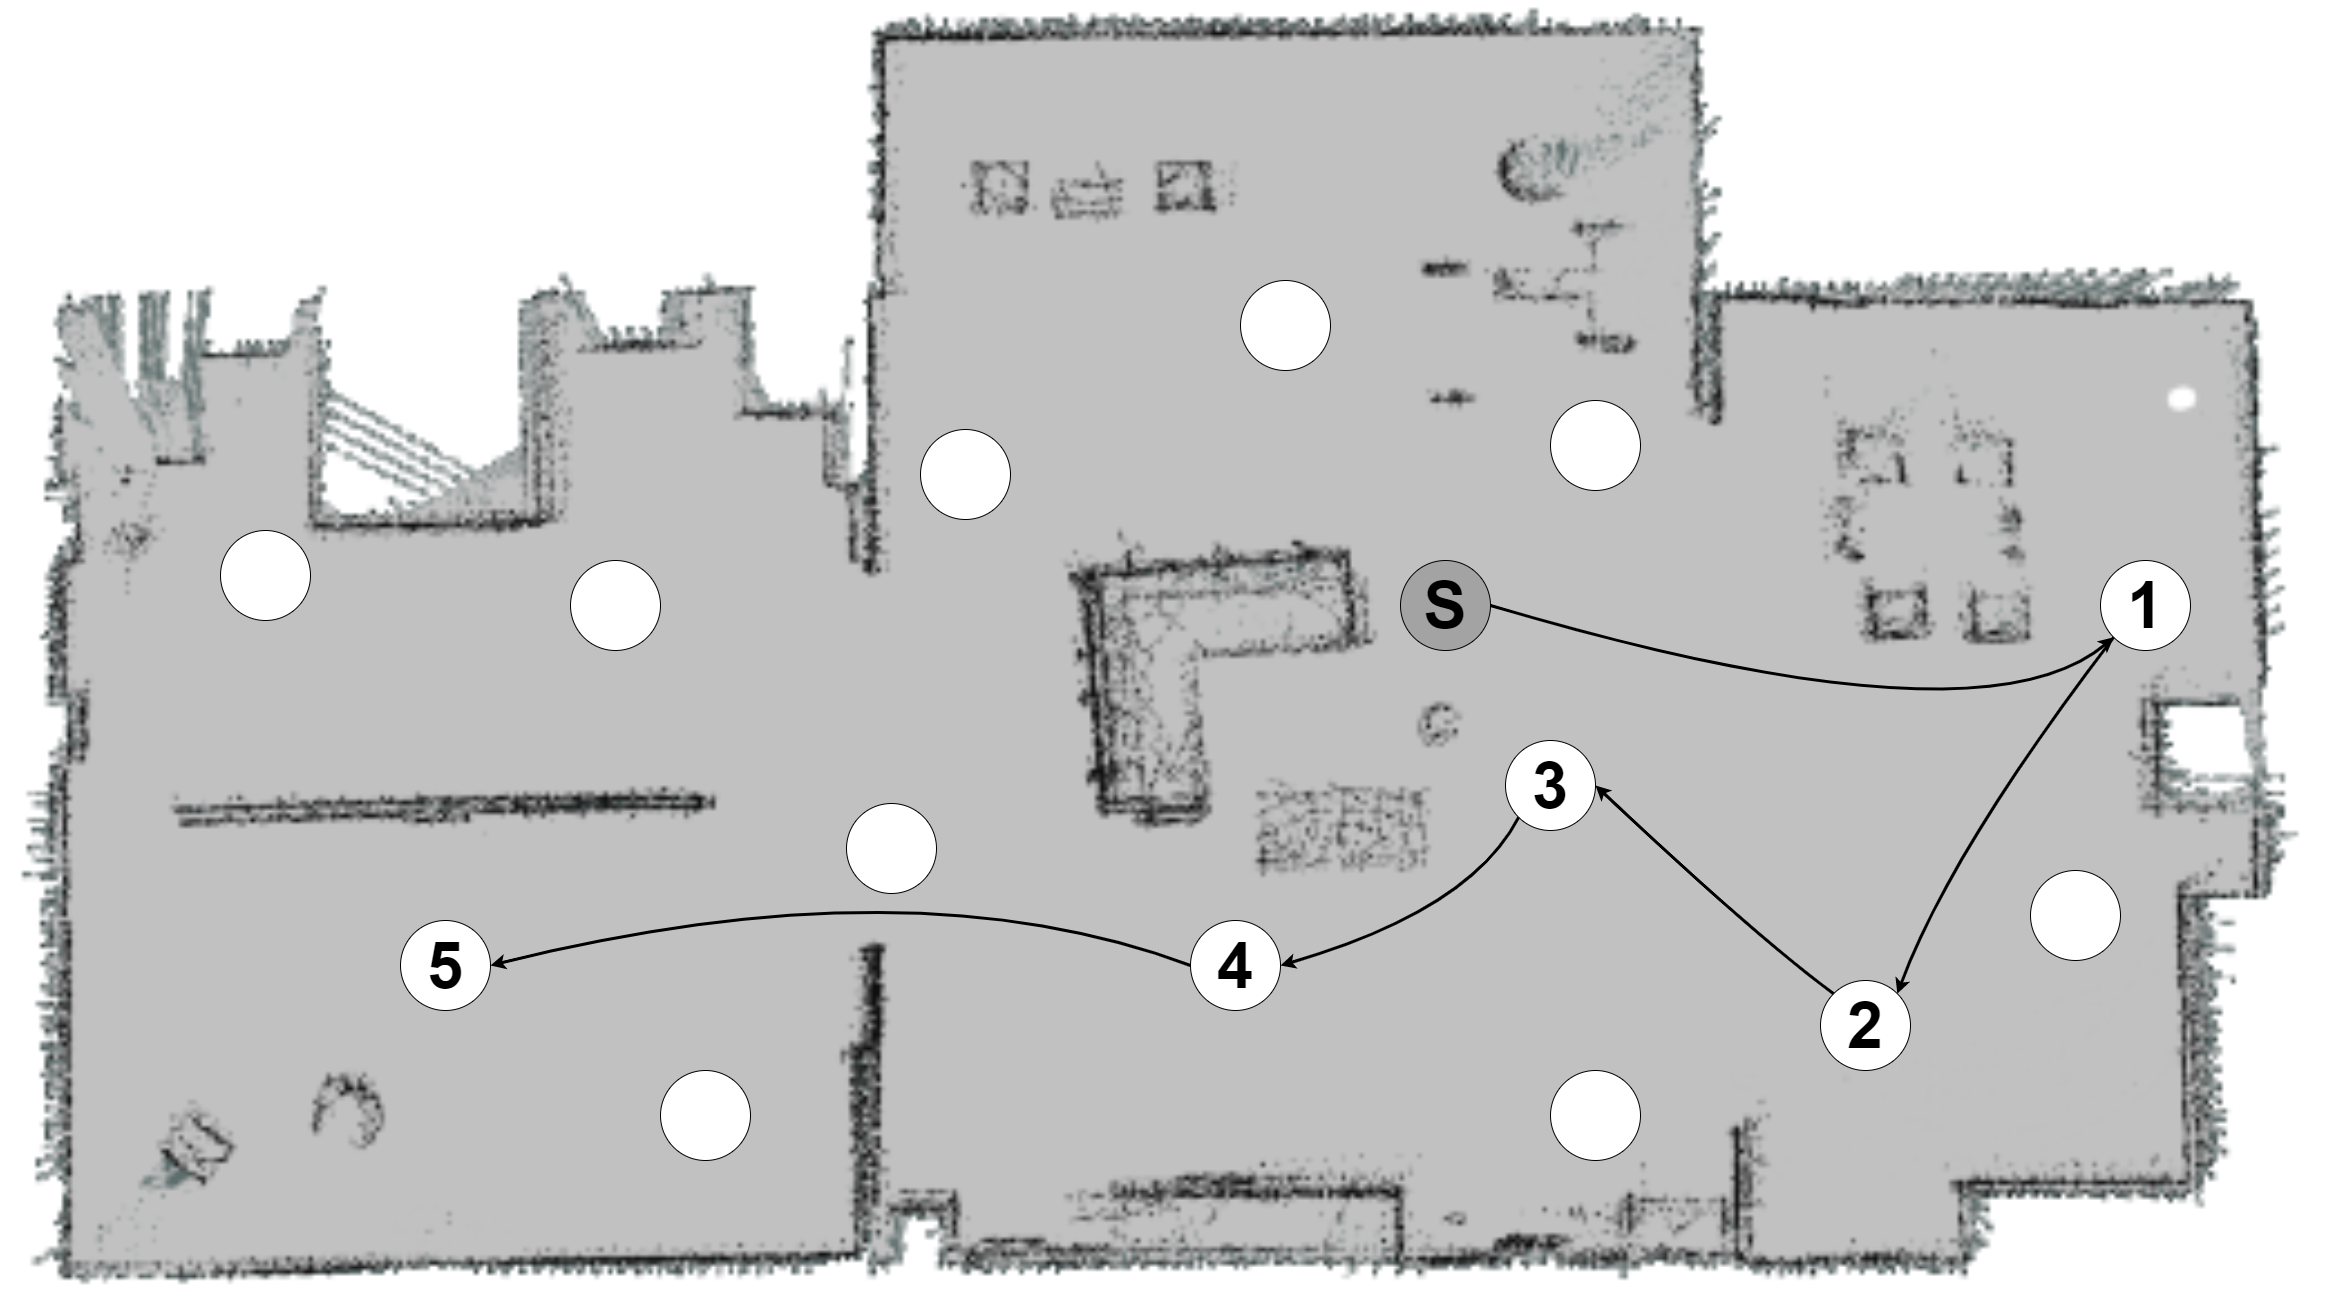
\includegraphics[width=0.5\textwidth]{Fig/消融c.png}
            \label{Ablationfigc}}\\
    \subfloat[LVL-Nav方法导航路径]{
            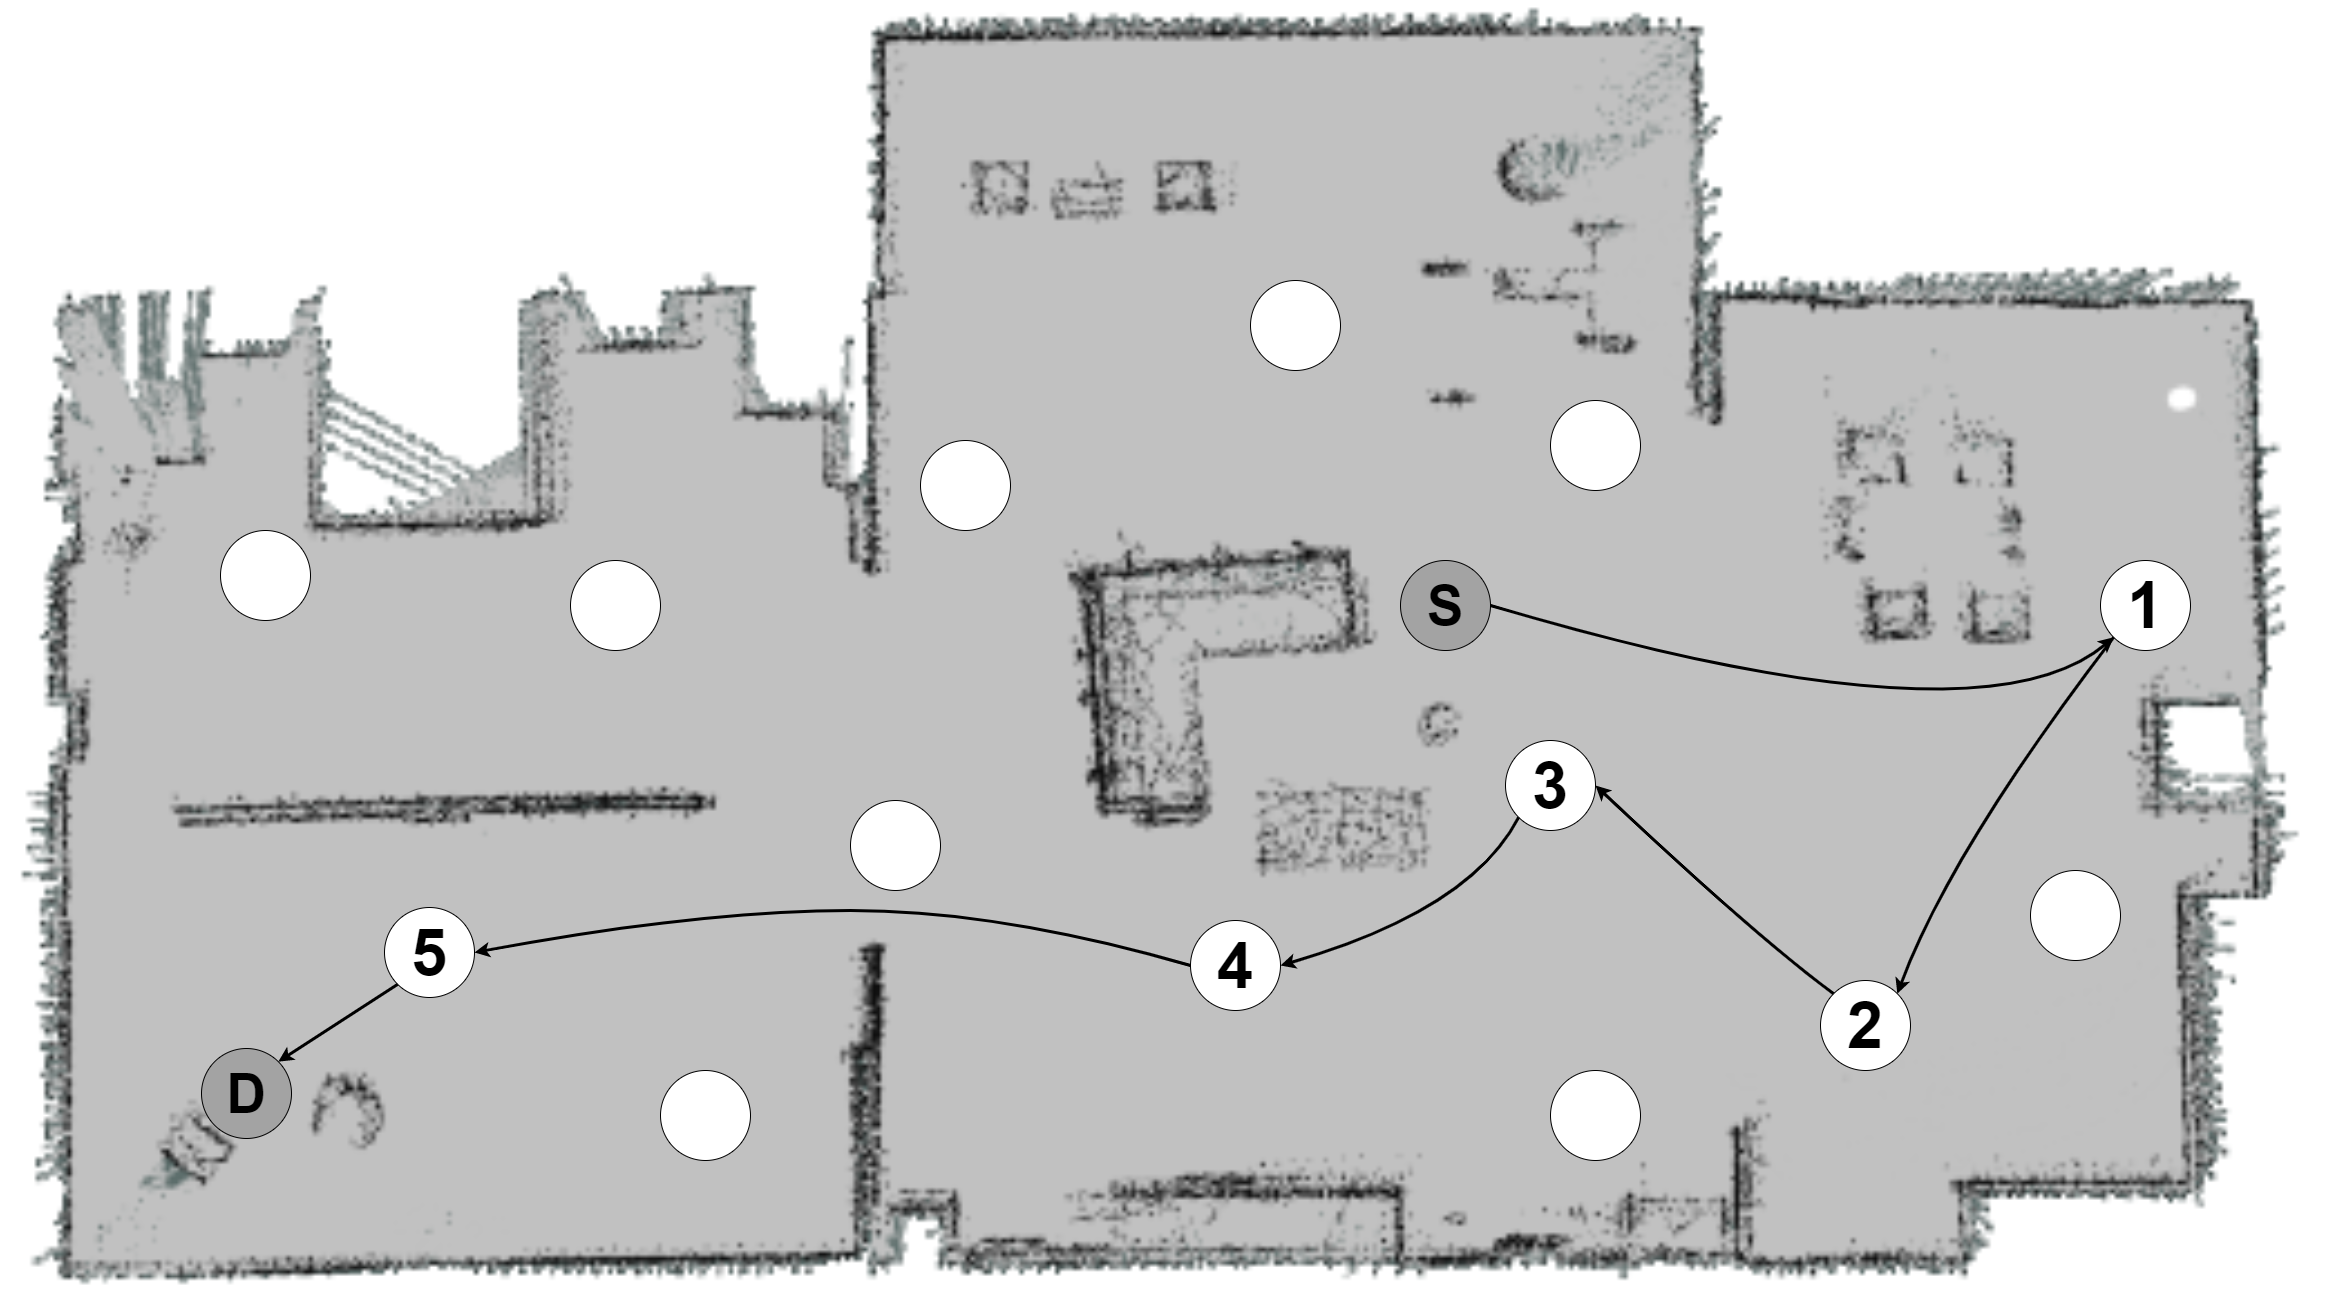
\includegraphics[width=0.5\textwidth]{Fig/消融d.png}
            \label{Ablationfigd}}
    \caption{消融实验结果}
    \label{Ablationfig}
\end{figure}
图中\ref{Ablationfiga}表示仅使用多模态融合网络根据五目标指令所执行的路径和导航到各子目标所捕获的图像,机器人无法利用环境中的距离和方位信息选取导航点、无法区分不同位置的相同目标,错误地选取了1、5两个相同导航点,且无法导航至目标半米内。
\ref{Ablationfigb}为仅使用多模态融合和导航点规划算法根据相同的五目标指令所执行的导航,机器人无法利用指令中的方位信息,错误地选择左前方最近的椅子作为第一个导航点。
\ref{Ablationfigc}为仅使用多模态融合、导航点规划和方位优化算法根据相同指令所执行的导航,移动机器人能够正确地通过多模态融合网络进行匹配,再利用导航点规划和方位优化进行筛选,得到了正确的导航点序列,但受限于导航点位姿的初始化,无法完成导航至目标半米内的任务。
\ref{Ablationfigd}为添加了局部路径规划方法所执行的正确导航,全局路径规划得到了正确的导航点序列,局部路径规划完成导航至目标半米内的任务。

对比仿真消融实验结果表明,本文所提出的多模态融合网络、导航点规划、方位优化和局部路径规划算法均能十分有效地帮助移动机器人理解指令目标、利用环境信息,使移动机器人能够根据指令高效且正确地执行导航。









\section{真实环境实验设计与评估}
由于仿真环境实验相对理想,移动机器人在导航的过程中不受过多传感器测量误差与其他外界因素干扰,且无法完全模拟真实机器人的计算性能,故需要真实环境实验进一步验证本文提出方法的有效性。
\subsection{实验设备}%多线激光、开发板参数、移动机器人整体
为进一步验证所提出算法在实际应用中的可行性,选用搭载了镭神C16激光雷达和杰锐微通HF899单目相机的灵遨移动机器人进行真实环境实验,其中激光雷达和用于进行导航实验的移动机器人如图\ref{C16laser}、\ref{mycar}所示。

\begin{figure}[h]
    \centering
    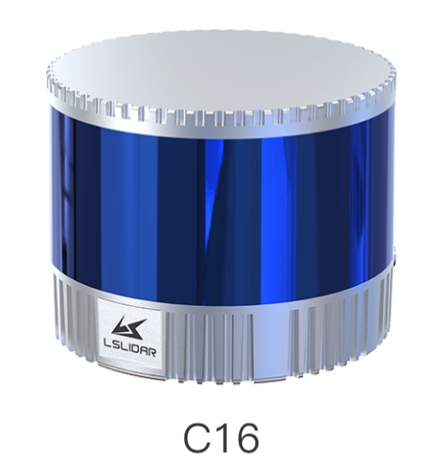
\includegraphics[scale=0.3]{Fig/C16laser.png}
    \caption{\label{C16laser}镭神C16激光雷达}
\end{figure}

\begin{figure}[htbp]
    \centering
    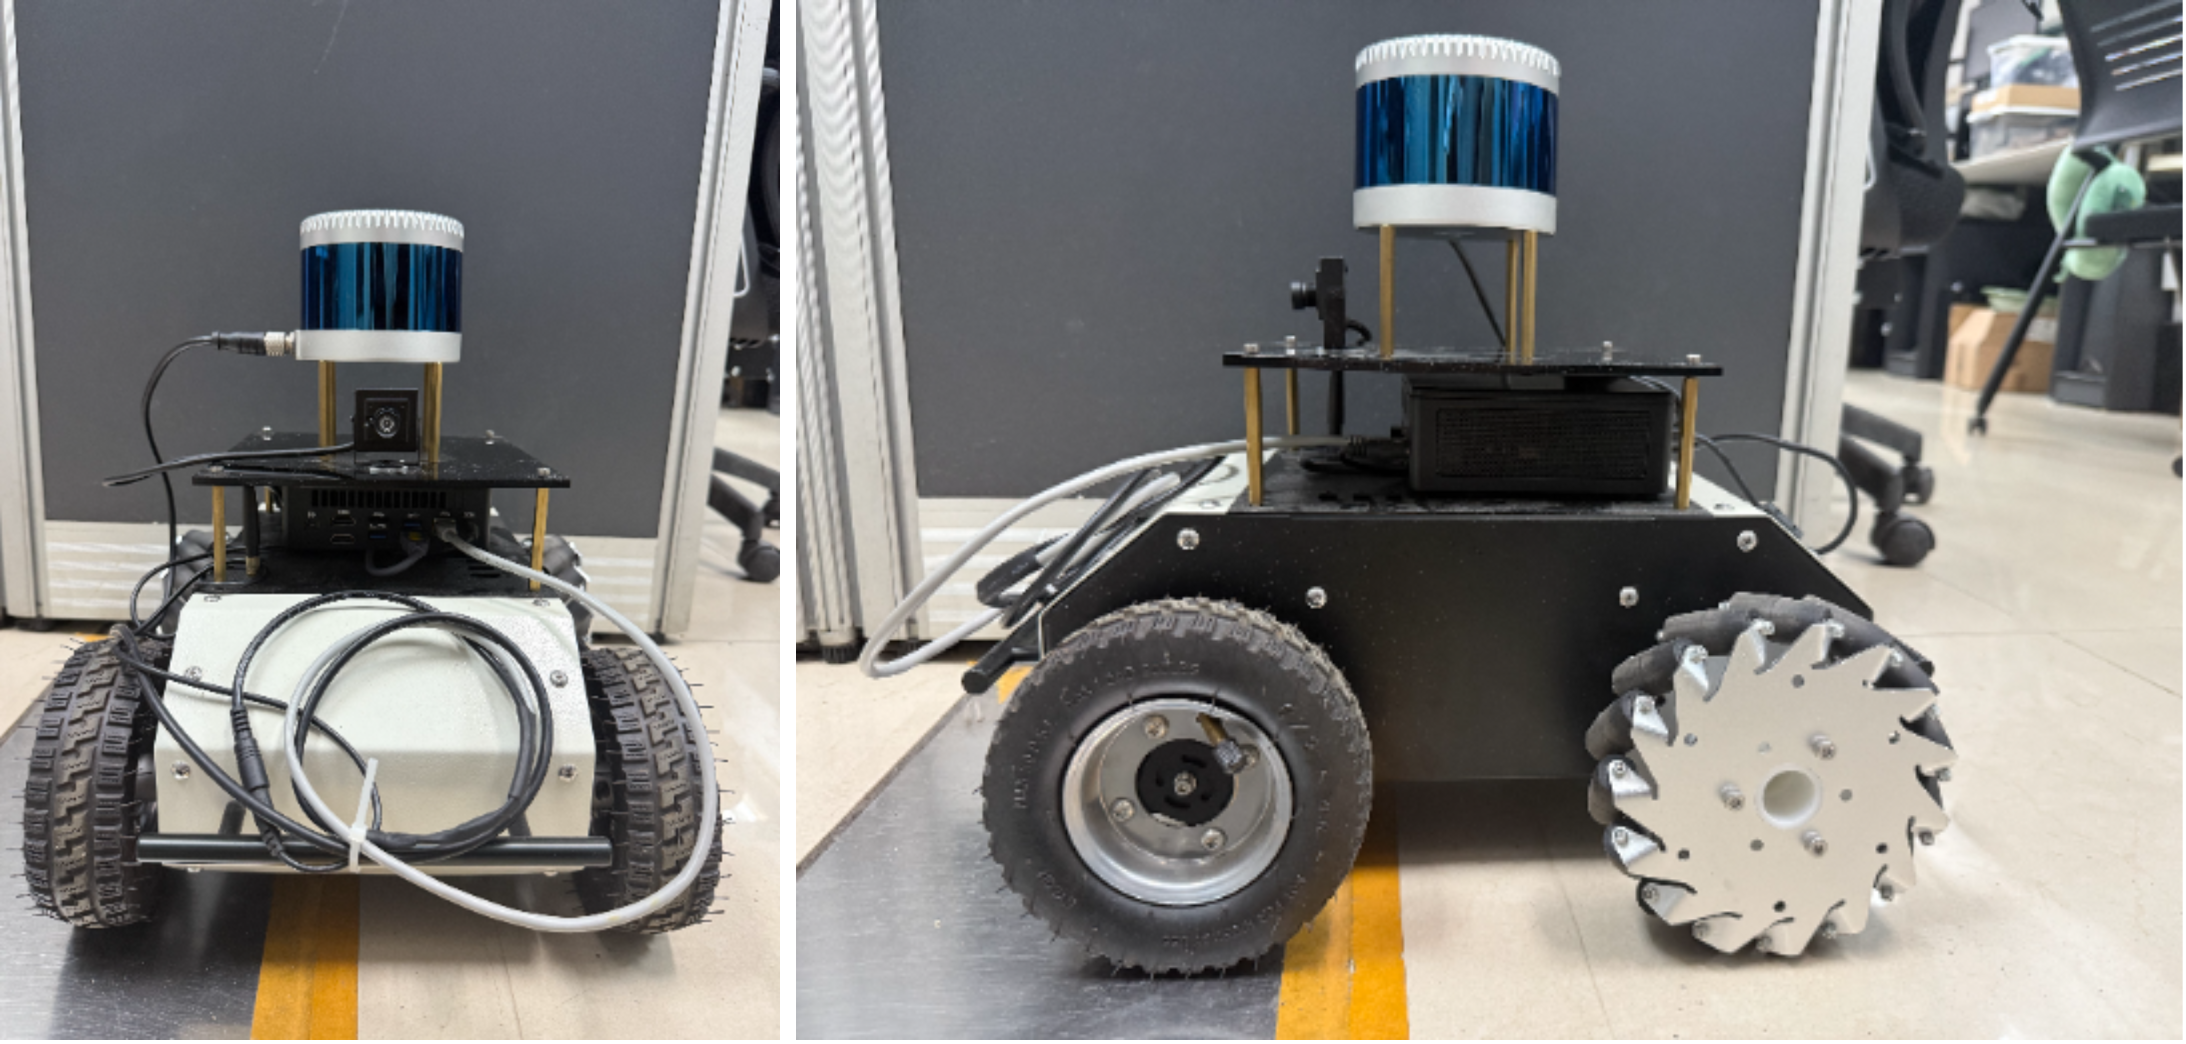
\includegraphics[scale=0.17]{Fig/robot.png}
    \caption{\label{mycar}灵遨移动机器人}
\end{figure}

如表\ref{hardcore}所示,我们将全局路径规划、ROS导航控制系统部署到UP Xtreme i11嵌入式开发板上;将局部路径规划中的特征提取、融合网络模型部署在Jetson TX嵌入式开发板上;灵遨机器人搭载码盘系统,通过IMU等装置实验机器人的移动;镭神C16激光雷达负责全局路径规划中的建图、导肮及局部路径规划中的图像点云融合;杰锐微通HF899单目相机负责局部路径规划中提供第一视觉视觉观察用于特征提取、融合和图像点云融合;其中UP Xtreme i11和Jetson TX嵌入式开发板如图\ref{boardfig}所示,设备的参数如表\ref{Embeddedboard}所示。
\begin{table}
    \caption{\label{hardcore}硬件系统设计}
    \centering
    \small
    \begin{tabular}{cc}
        \hline
        设备 & 功能 \tabularnewline 
        \hline 
        UP Xtreme i11 & 部署全局路径规划、驱动机器人 \tabularnewline
        Jetson TX & 部署导航模型进行探索推理 \tabularnewline
        灵遨机器人 & 移动机器人 \tabularnewline
        镭神C16激光雷达 & 建图、导航及图像点云融合 \tabularnewline
        杰锐微通HF899单目相机 & 获取视觉观察 \tabularnewline
        \hline 
    \end{tabular}
\end{table}


\begin{figure}[h]
    \centering
    %\includegraphics[width=3in]{fig5}
    \subfloat[UP Xtreme i11]{
            \includegraphics[scale=0.071]{Fig/up.jpg}}
    \subfloat[Jetson TX]{
            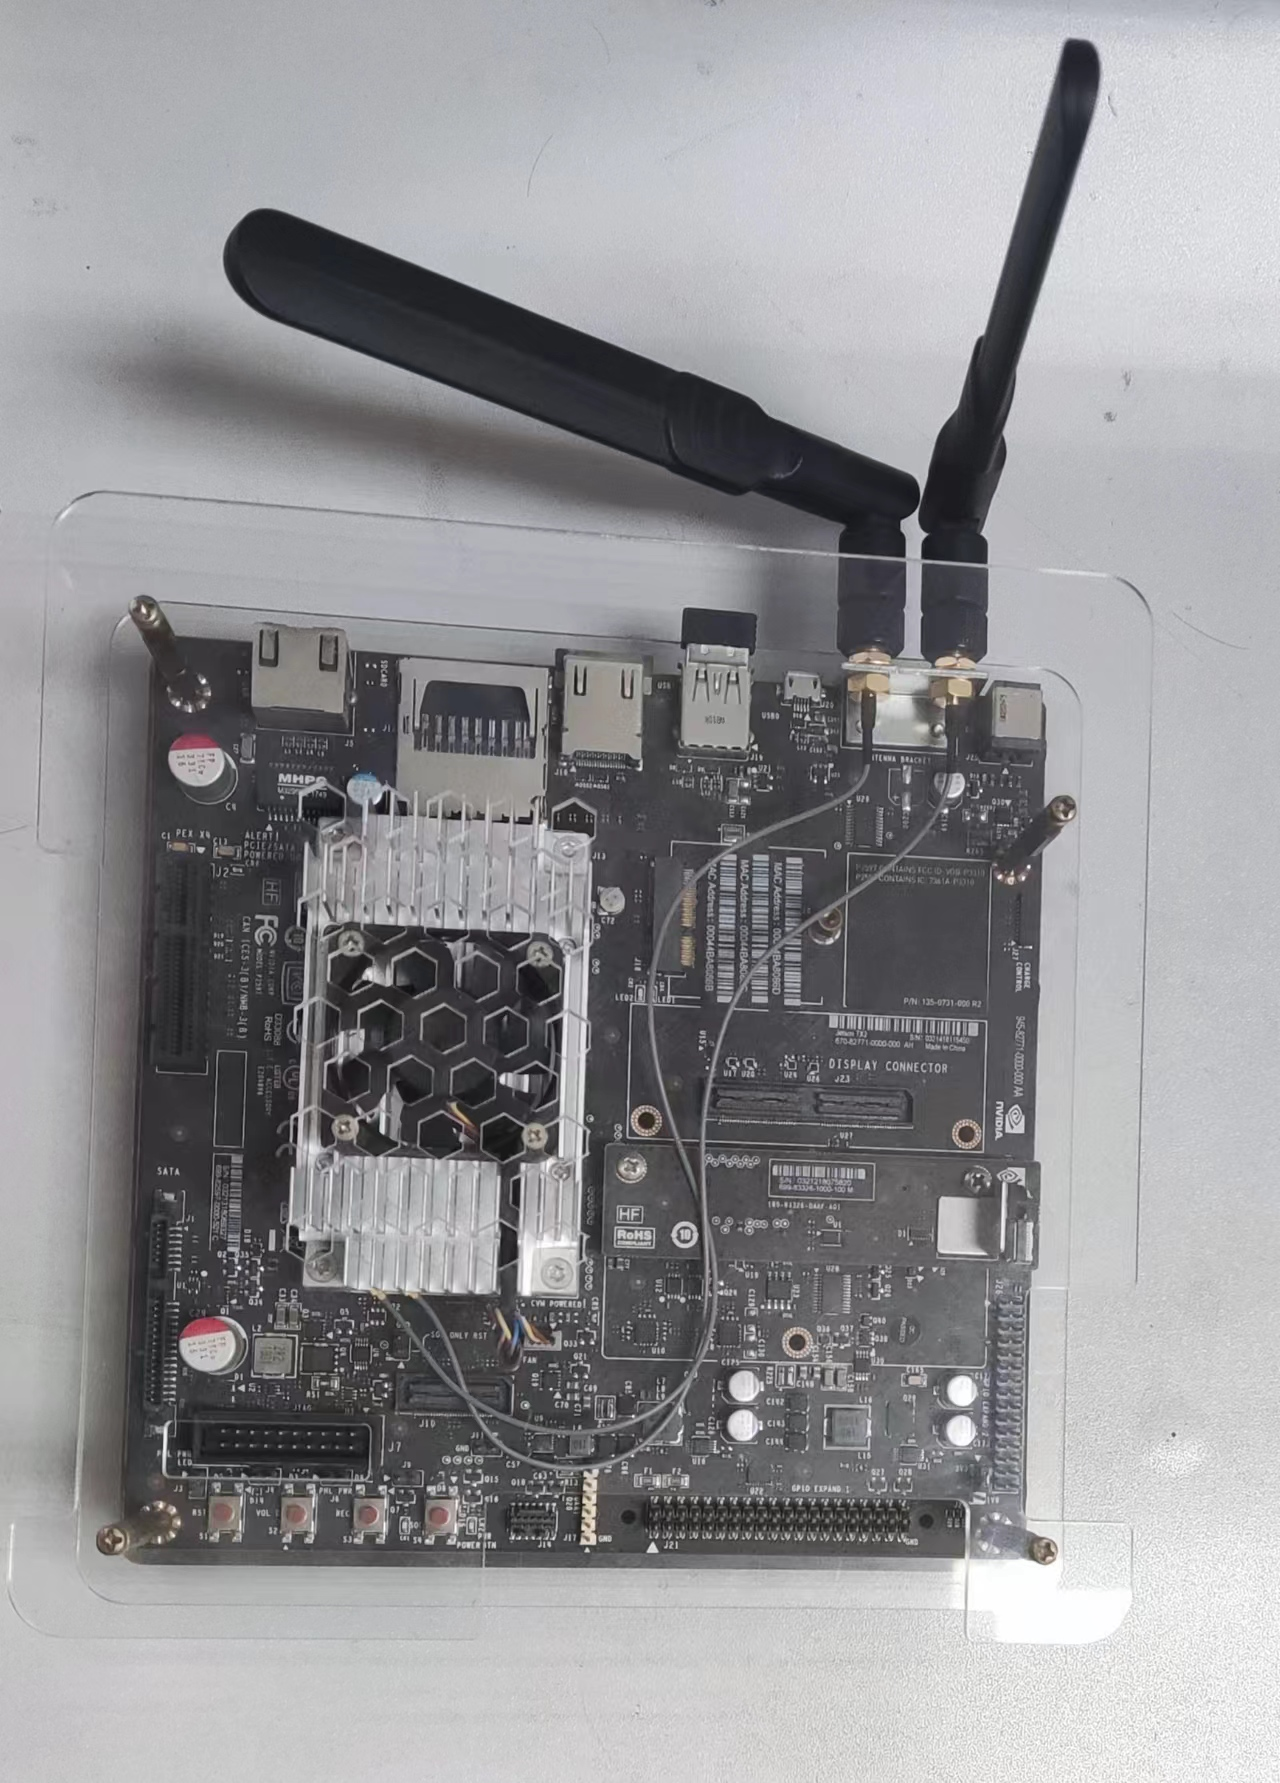
\includegraphics[width=0.34\textwidth]{Fig/Jetsonfig.png}}
    \caption{嵌入式开发板}
    \label{boardfig}
\end{figure}


\begin{table}[]
    \caption{\label{Embeddedboard}硬件设备参数}
    \centering
    \begin{tabular}{c|c|c}
    \hline
    软硬件  & UP Xtreme i11                               & Jetson TX2                                                                                                               \\ \hline
    GPU  & Intel(R)Iris(R) Xe Graphics                 & 256-core NVIDIA Pascal architecture GPU                                                                                  \\
    CPU  & 11th Gen intel r core(tm) i7-1165G7 & \begin{tabular}[c]{@{}c@{}}Dual-core NVIDIA Denver 2 64-bit CPU\\ Quad-core Arm Cortex-A57 MPCore processor\end{tabular} \\
    AI性能 & 1.0TFLOPS                                   & 1.33TFLOPS                                                                                                               \\
    内存   & 2GB                                         & 8GB                                                                                                                      \\
    存储   & 24GB                                        & 32GB                                                                                                                     \\
    功率   & 65w                                         & 7.5w-15w                                                                                                                 \\ \hline
    \end{tabular}
    \end{table}



\subsection{实验环境}
本文的真实实验场景搭建在学院楼内的实验室,总面积约有45平方米。实验场景包含成排的桌子、一个饮水机、一个打印机、一个冰箱、两个书架、几张椅子,布局设计成室内办公桌的样式,真实实验环境及其栅格地图如图\ref{myrealenv}所示。我们从32个室内常见物体中随机选择多个连续的指令目标在真实环境中进行实验,包括冰箱、打印机这种不存在复数的目标,也包括椅子、笔记本电脑等这种存在复数的目标。
\begin{figure}[h]
    \centering
    %\includegraphics[width=3in]{fig5}
    \subfloat[真实实验环境]{
            \includegraphics[width=0.70\textwidth]{Fig/realenv.jpg}}\\
    \subfloat[真实实验环境栅格地图]{
            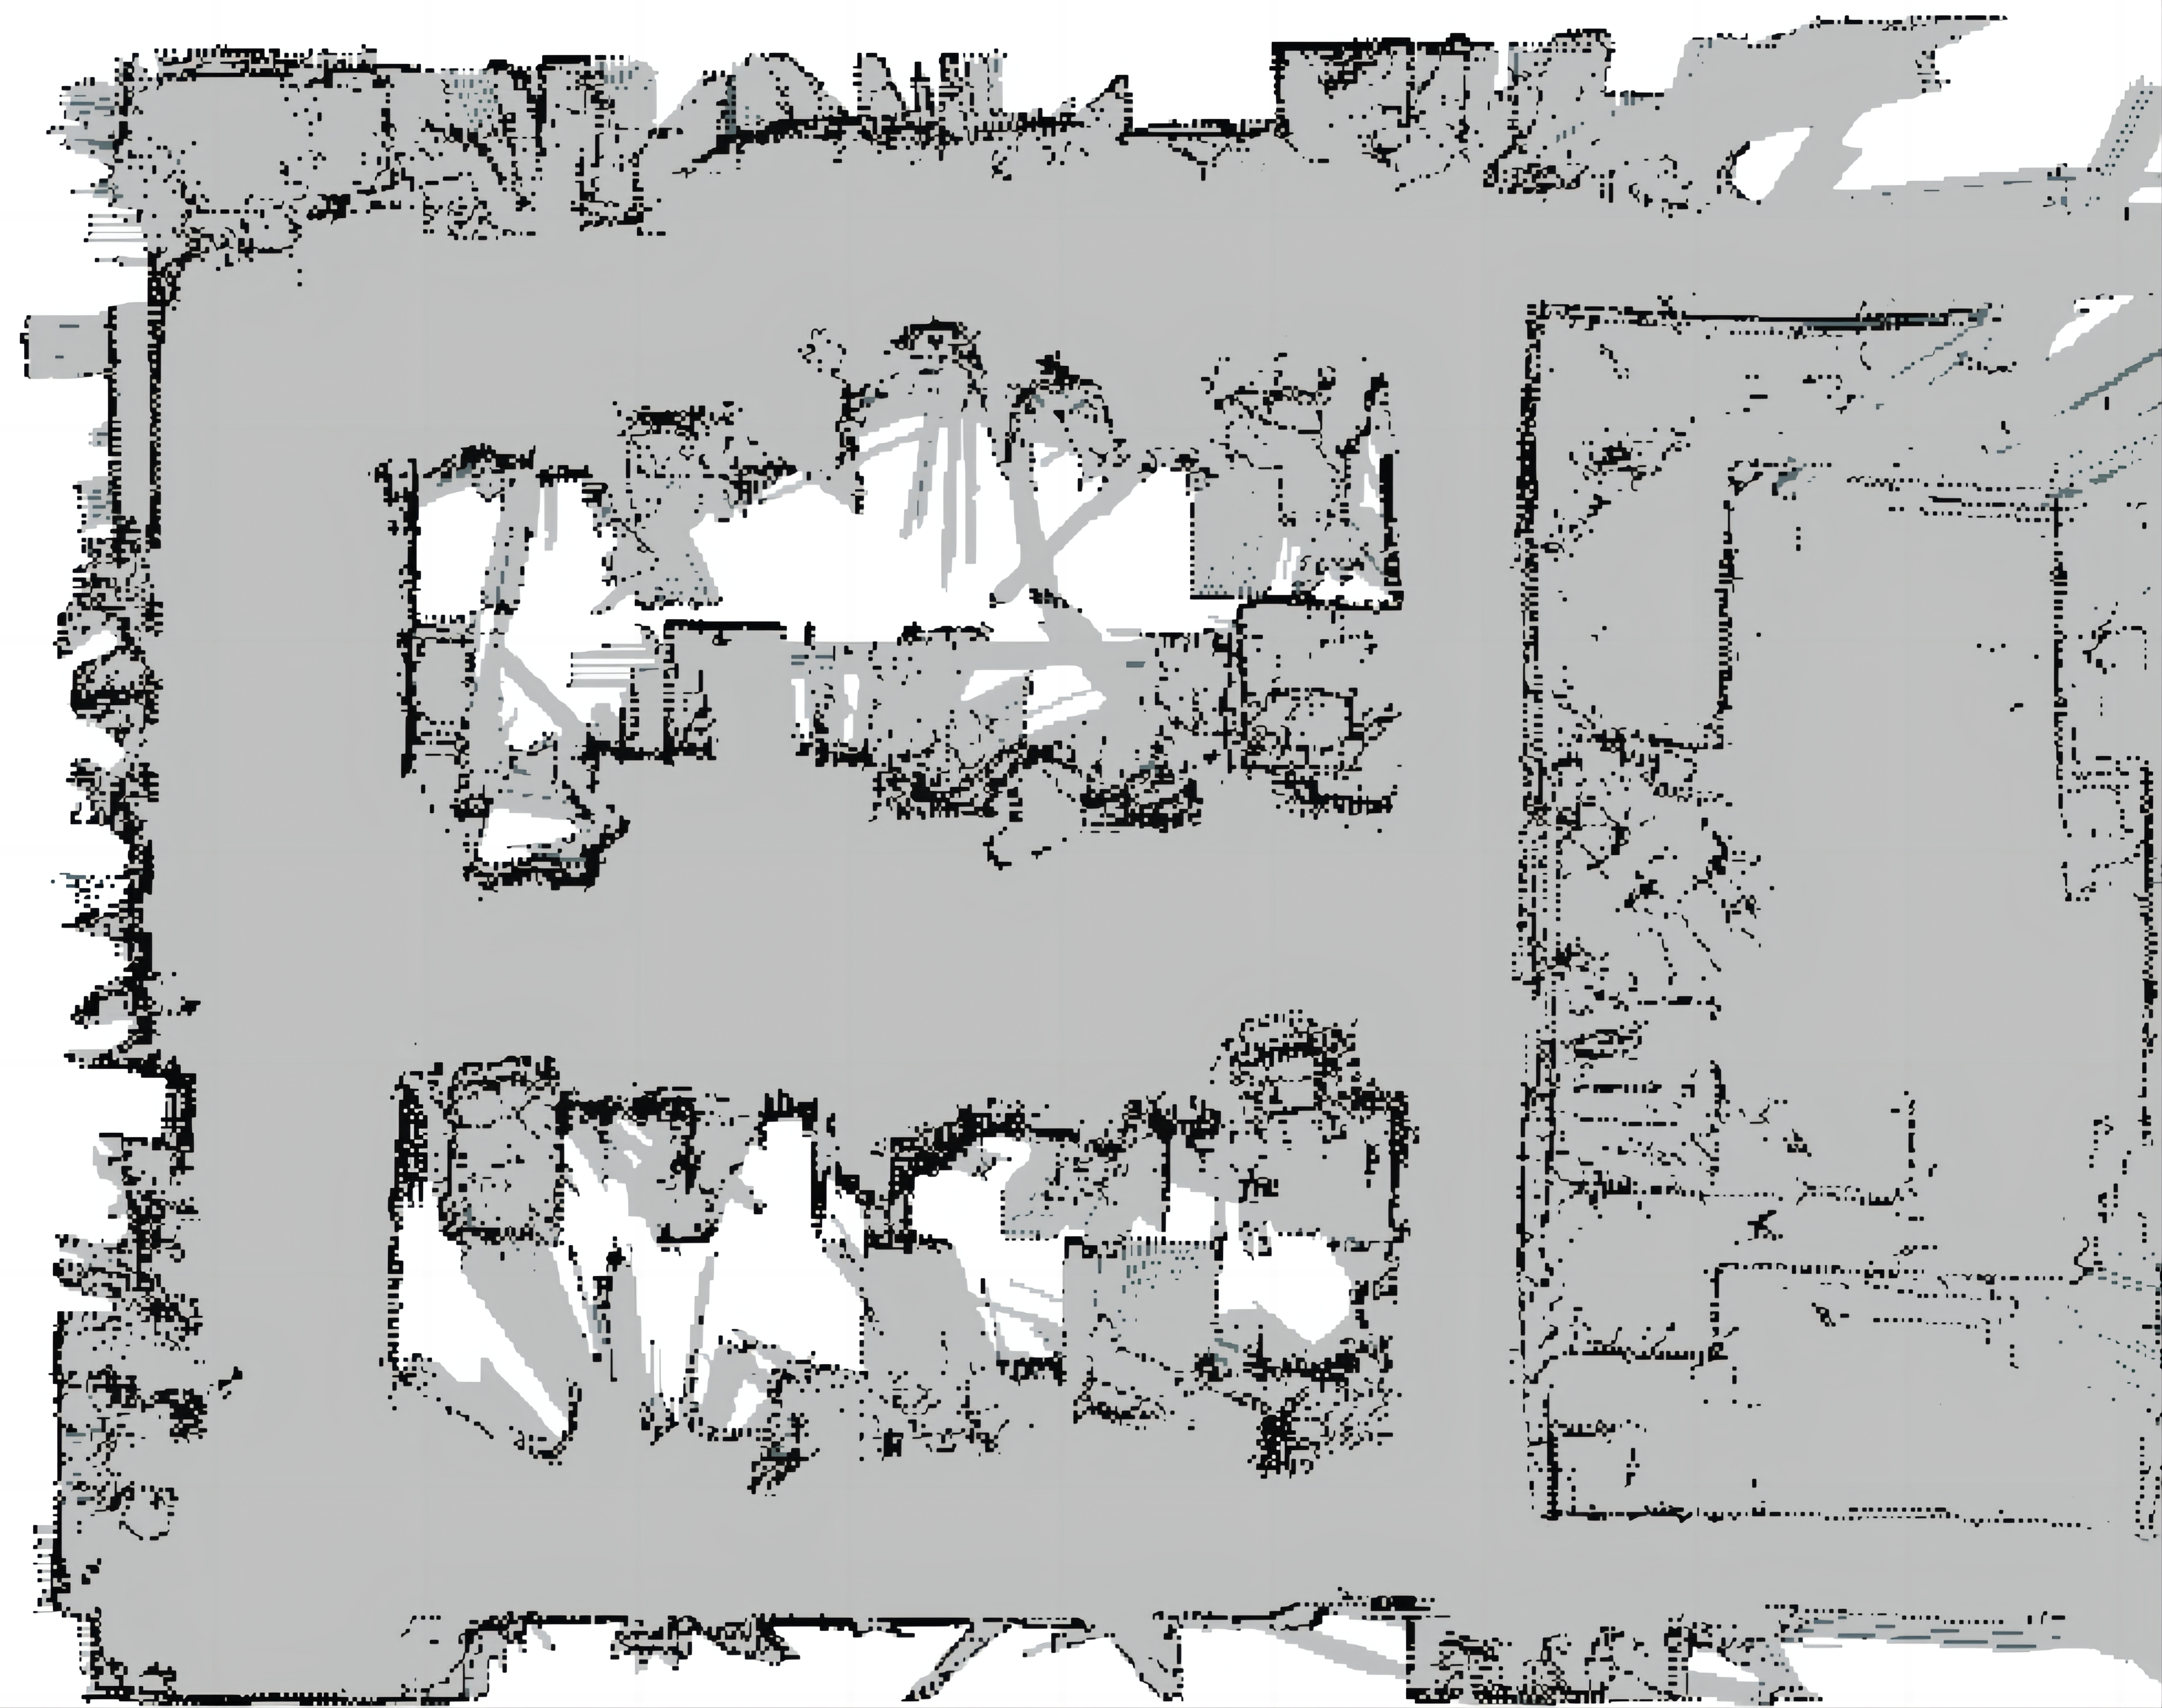
\includegraphics[width=0.70\textwidth]{Fig/realenvmap.jpg}}
    \caption{真实环境}
    \label{myrealenv}
\end{figure}
真实环境中的实验直接使用仿真环境中由全局路径规划和局部路径规划共同构成的LVL-Nav方法进行测试,不在现实测试环境中采集数据来重训练模型,同时也不改变各算法参数,以此来验证所提出的方法在真实环境下的迁移效果,并找出方法的优势和局限。

真实实验的运行环境为内存16GB的64位Ubuntu18.04操作系统,平台为ROS Melodic。通过局域网完成网络连接配置后,使用笔记本电脑执行远程操作,控制机器人完成建图、记录导航点与图像并根据指令执行导航。
在实验的设计上,本文采用随机抽取并随机排序的方法在上述的目标物体中进行选择,在实验环境中也随机布局这些被选中的物体。当移动机器人的局部路径规划在执行完成图像点云融合算法并输出"导航结束"时作为移动机器人完成一次导航的信号,若在导航的过程中正确地根据指令经过所要求的所有目标,并在最后的目标半米内停止则表示本次真实环境下的导航成功,除此之外,在整个导航的过程中若发生过碰撞或导航超时则都判定为导航失败。



\subsection{导航实验}
\begin{figure}[h]
    \centering
    \subfloat[激光点云可视化]{
            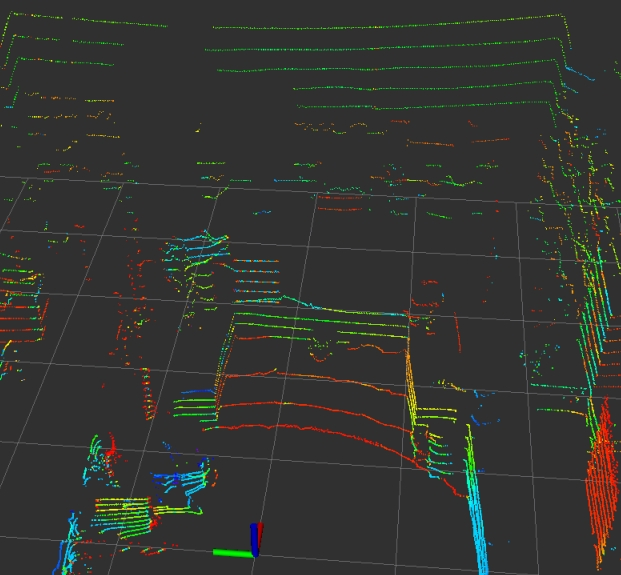
\includegraphics[width=0.65\textwidth]{Fig/laserfusion.png}}\\
    \subfloat[融合效果图]{
            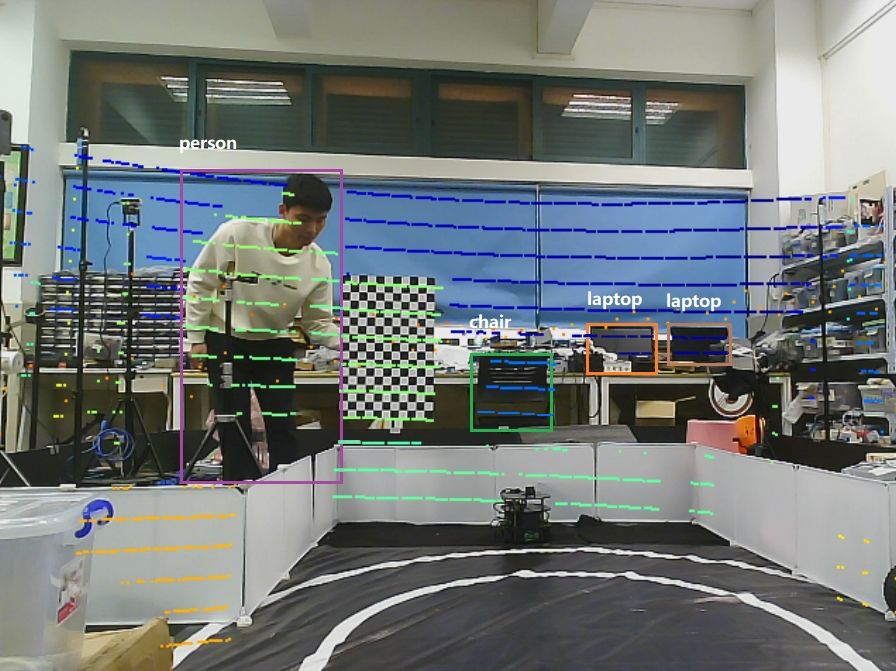
\includegraphics[width=0.65\textwidth]{Fig/fusion.png}}
    \caption{图像点云融合可视化}
    \label{myfusion}
\end{figure}
实验中先将单目相机和激光雷达通过张正友标定法进行联合标定,得到的外参数据如式\ref{myeqcor}所示,我们发现仅依靠由多模态融合、导航点规划和方位优化组成的全局路径规划已经能较为可靠地依照自然语言指令进行导航点匹配,但仍然存在指令目标移动导致目标不在导航点旁的情况,从而导致仅依靠全局路径规划导航任务的失败。局部路径规划可以在局部环境中通过将视觉观察进行特征融合、特征提取进而实现探索,当目标出现在视觉观察中时可以在图像点云融合模块中结合目标检测、点云聚类和坐标变换方法将空间点云数据映射到视觉图像之中,映射结果如图\ref{myfusion}所示,包括来自于图像目标检测结果的物体分类信息和来自于十六线激光雷达通过聚类后物体相对于激光源的距离信息,如若指令需要导航到目标“person”的附近,代理则会在局部探索到目标后融合的结果将点云平均距离作为目标与移动机器人之间的实际距离,再根据平面成像原理依次计算出目标在机器人坐标系和map坐标系下的具体位姿。
最终通过发布导航任务以完成局部路径的规划,实现导航到目标半米内的闭环任务。
\begin{equation}
    R = \left[ {\begin{array}{*{20}{c}}
{ - 0.0419}&{0.0487}&{0.9979}\\
{ - 0.9985}&{ - 0.0379}&{ - 0.0401}\\
{0.0359}&{ - 0.9981}&{0.0502}
\end{array}} \right],t = \left[ {\begin{array}{*{20}{c}}
{0.1549}\\
{ - 0.0253}\\
{0.0952}
\end{array}} \right]
    \label{myeqcor}
\end{equation}




为了验证本文所提出方法在复杂多变真实环境中依照指令进行导航的能力,我们给定只在方位和目标上存在细微差距的五目标导航指令进行实验,如图\ref{realenvsuccess}和\ref{realenvfalied}所示。
\begin{figure}[htbp]
    \centering
    \includegraphics[width=0.85\textwidth]{Fig/realsuccess.png}
    \caption{\label{realenvsuccess}真实环境成功导航示例}
\end{figure}

\begin{figure}[htbp]
    \centering
    \includegraphics[width=0.85\textwidth]{Fig/realfalied.png}
    \caption{\label{realenvfalied}真实环境失败导航示例}
\end{figure}

前者是一次真实环境成功导航示例,学院楼实验室的门口出发,根据全局路径规划获得的目标导航点之后,在ROS中发布目标位姿依次进行目标物体导航,在直行经过储物柜之后移动机器人根据匹配的目标点继续导航到前方的冰箱旁,然后右转依次经过书架和风扇这两个导航点,接着得益于全局路径规划中的方位优化和多模态融合网络,在最后目标椅子的导航点选择中代理不会错误地选择在环境中离自己最近的风扇旁的其他椅子,而是前往指令要求的前方最近的椅子,从而正确匹配离工作台椅子旁最近的导航点,最后根据局部路径规划中的特征提取融合和运动模块在视觉观察中进行探索,检测到最终目标后通过图像点云融合模块获得环境中椅子的真实位姿,发布位姿后执行以顺利完成导航任务。

后者是一次真实环境失败导航示例,我们特意选用只具有细微差别但完全不同的导航指令来测试代理理解指令并正确执行导航的能力,所以同样地在学院楼实验室的门口出发,根据全局路径规划获得的目标导航点之后,在ROS中发布目标位姿依次进行目标物体导航,在直行经过储物柜之后根据方位指示前往右方,在经过有很多椅子较为狭窄的环境后导航到双肩背包旁,接着左转经过摆放着水杯的桌角导航到同一个风扇旁,但经过我们的实验发现,移动机器人在50cm这种十分狭窄的环境中无法跨过风扇脚驶出狭窄环境,最终在通道里调整姿态并因为导航超时导致导航失败,这是由于在真实的室内环境存在大量不变移动变化的障碍物,这导致移动机器人无法十分有效地在狭窄的环境中进行可靠地导航。



本文在真实实验场景中针对不同的自然语言导航指令一共实验了20次,目标物体从“mouse”“laptop”等室内常见物体中进行随机选择,而目标物体则摆放在真实场景中的随机可见位置,在实际的导航过程中目标物体导航总体成功率约为50\%。
真实环境下的实验结果表明本文提出的导航方法以可靠且高效地根据任意形式的自然语言指令和环境拓扑信息,在光照条件变化大的复杂室内环境中融合感知和认知信息正确规划出全局路径,具备区分导航指令中的细微方向、目标差别的能力,同时局部路径规划允许移动机器人不依赖于环境中导航点位置的设置,使其能够正确的导航到目标半米内。

另一方面,我们在测试的过程中也发发现了方法中的不足之处。由于真实环境和仿真环境的差异问题导致了局部路径规划中的特征提取、融合模型性能的下降,当目标未能出现在移动机器人的视觉观察之中时,局部探索方法在存在遮挡物体的环境中存在失败的可能从而导致导航的失败;并且由于真实的室内环境摆放大量的障碍物,这导致移动机器人无法十分有效地在狭窄的环境中进行可靠地导航,在与椅角或桌角发生碰撞后无法继续导航从而导致导航的失败。


\section{本章小结}

本章主要介绍了本文所提出的语言视觉激光多模态融合的机器人导航方法在仿真、真实环境进行目标物体导航的实验,我们通过和近三年表现良好方法的对比试验验证了本文所提出方法的有效性,即通过引入深度信息优化多模态融合网络,提高模型在光线条件变化大的室内的鲁棒性;提出了一种方位优化法筛选不符合方位条件的冗余导航点;通过导航点规划算法进一步提高全局路径规划所生成导航点的正确率;设计了一种特征提取、融合网络能够有效地在局部未知环境中进行探索,设计并实现了一种单目相机和多线激光传感器融合的局部导航方法以完成导航至目标半米内的闭环任务;通过消融实验分析并验证了所提出方法中各个模块的有效性。

实验结果表明,我们所提出的方法在仿真、真实环境中的导航表现基本达到了预期,但受限于真实、仿真环境之间的差异以及真实狭窄环境对局部探索导航和基于目标点导航两方面的影响,移动机器人在真实环境中也存在导航失败的问题亟待解决。